\chapter[Appendix to DeepPoseKit]{Appendix to ``DeepPoseKit: a software toolkit for fast and robust animal pose estimation using deep learning"}
\newpage
    \label{app:figures}
    \begin{figure}[!htb]
    
    \centering
    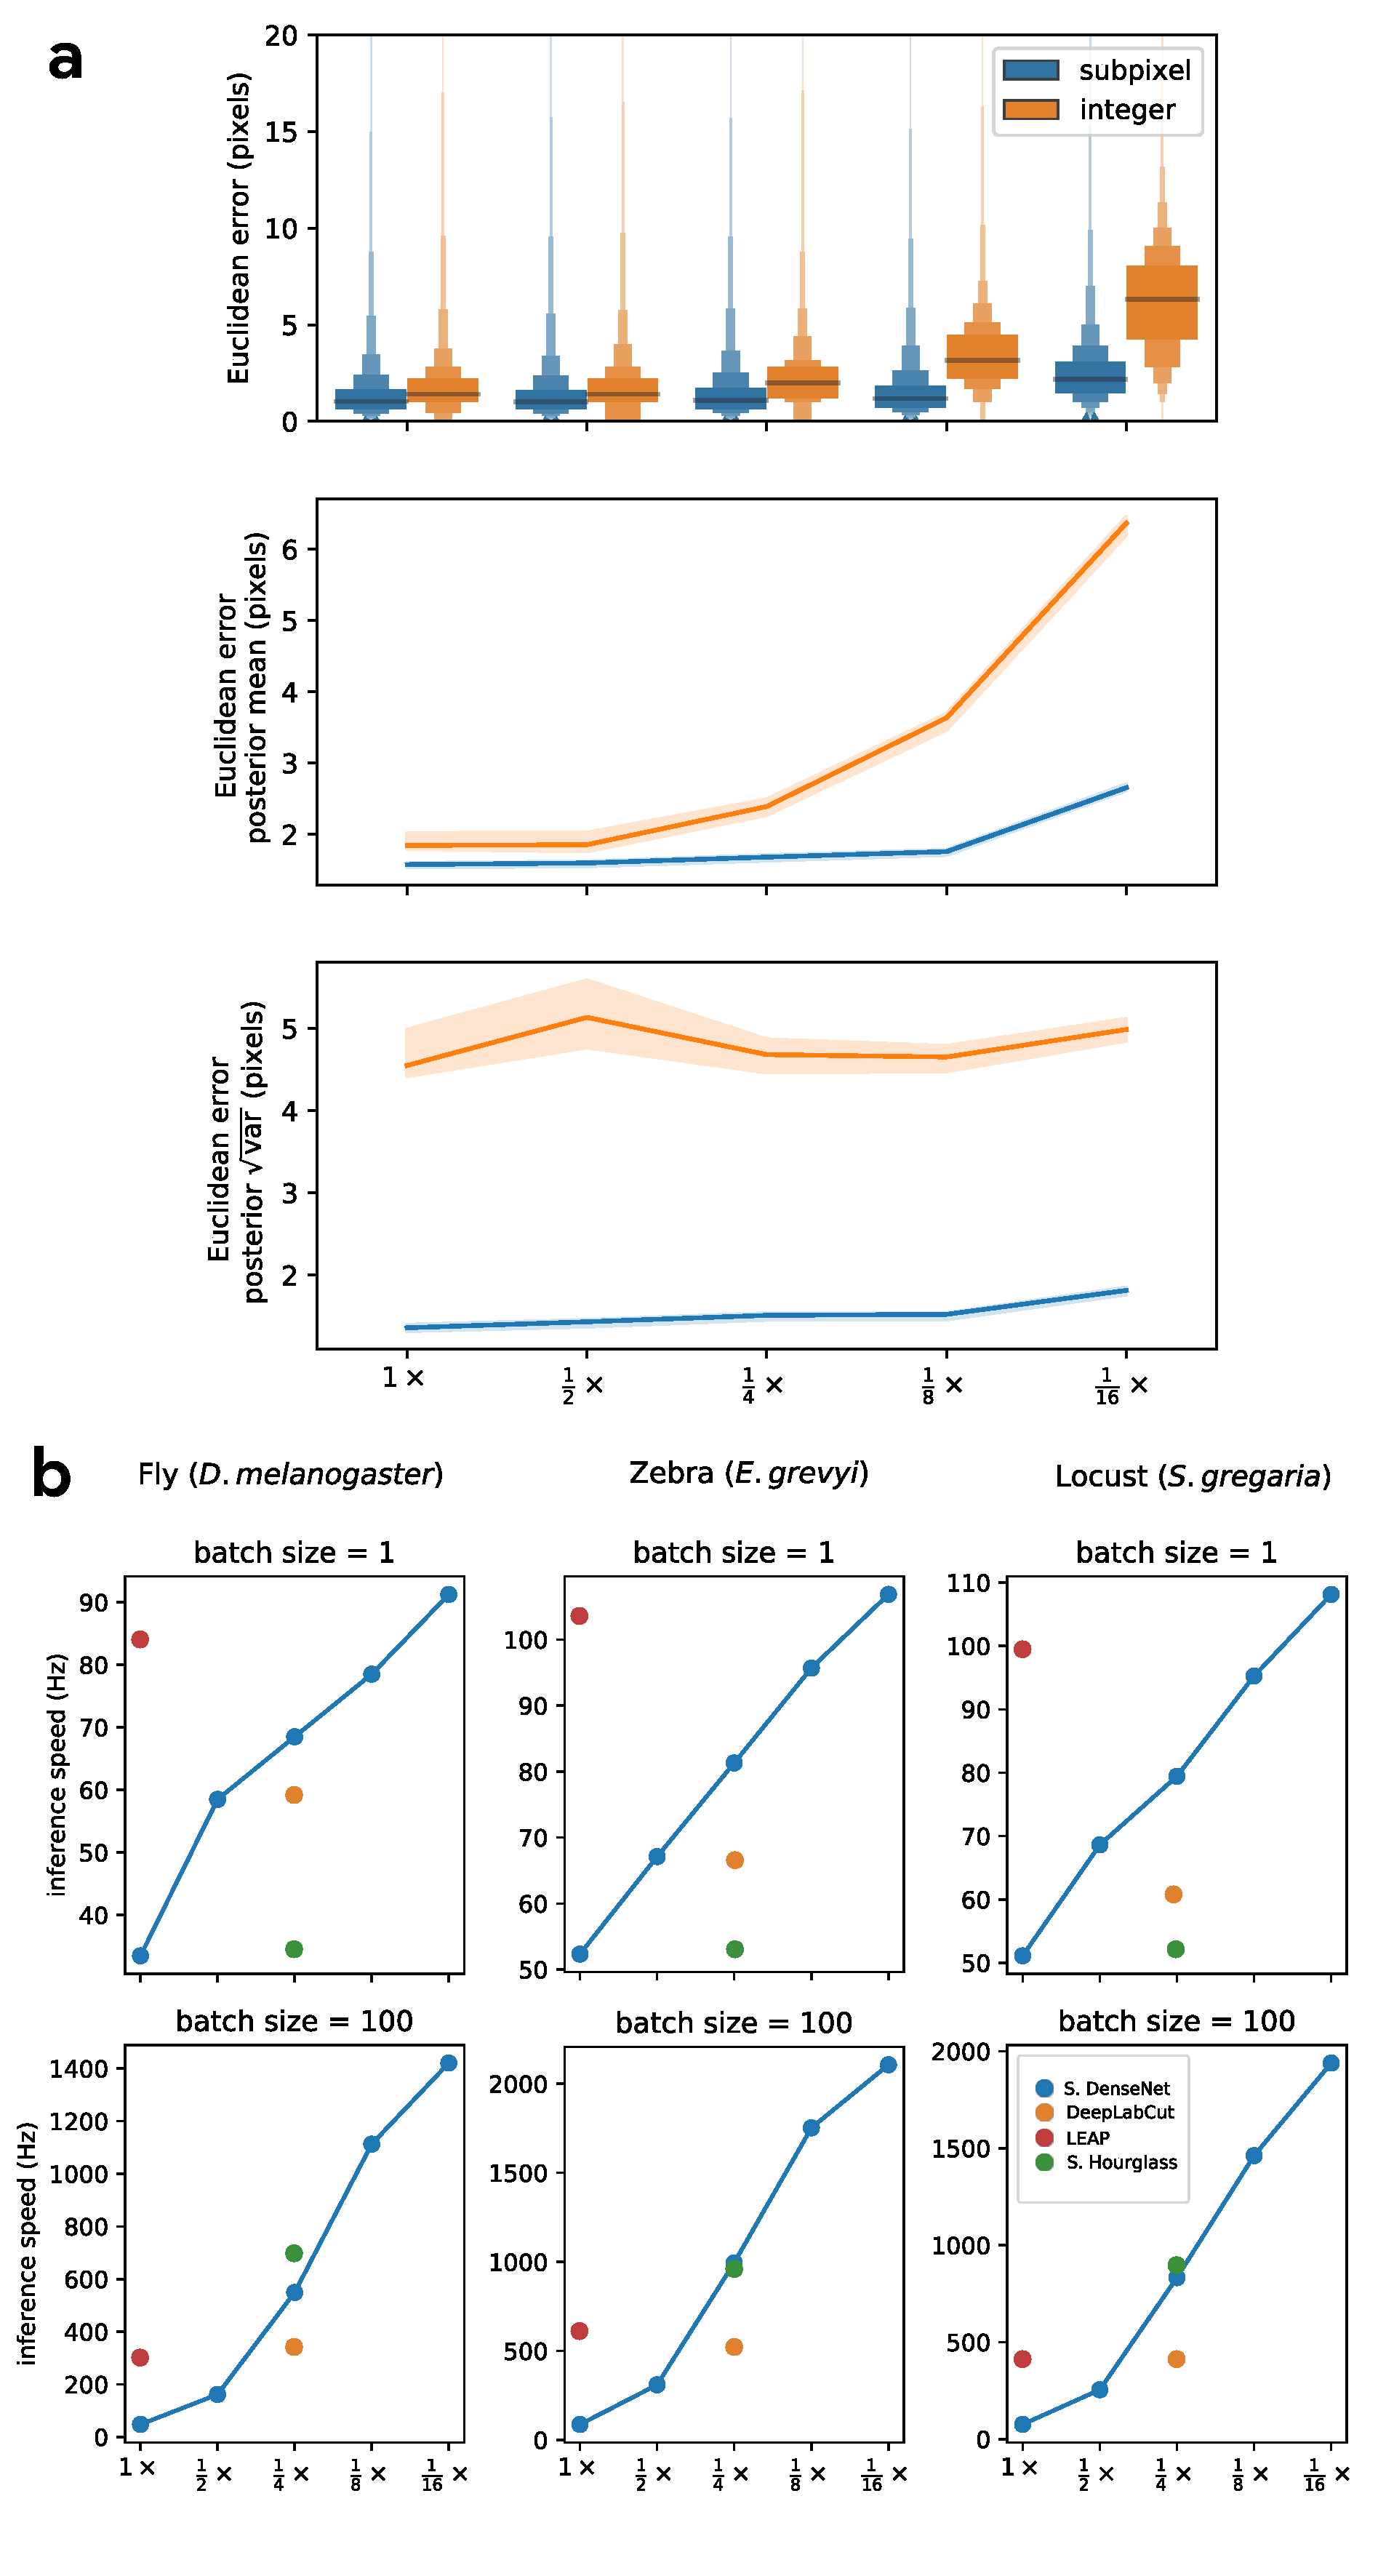
\includegraphics[width=0.60\linewidth]{Graving_IMPRS_Thesis/figures/downsample_inference_speed.pdf}
    \caption{Our subpixel maxima algorithm increases speed without decreasing accuracy. Prediction accuracy on the fly dataset is maintained across downsampling configurations (\textbf{a}). Letter-value plots (\textbf{a-top}) show the raw error distributions for each configuration. Visualizations of the credible intervals (99\% highest-density region) of the posterior distributions for the mean and variance (\textbf{a-bottom}) illustrate statistical differences between the error distributions, where using subpixel maxima decreases both the mean and variance of the error distribution. Inference speed is fast and can be run in real-time on single images (batch size = 1) at $\sim$30-110Hz or offline (batch size = 100) upwards of 1000Hz (\textbf{b}). Plots show the inference speeds for our Stacked DenseNet model across downsampling configurations as well as the other models we tested for each of our datasets. }
    \label{fig:downsample_inference_speed}
    
    
    \end{figure}
    
    \begin{figure}[!htb]
    
    \centering
    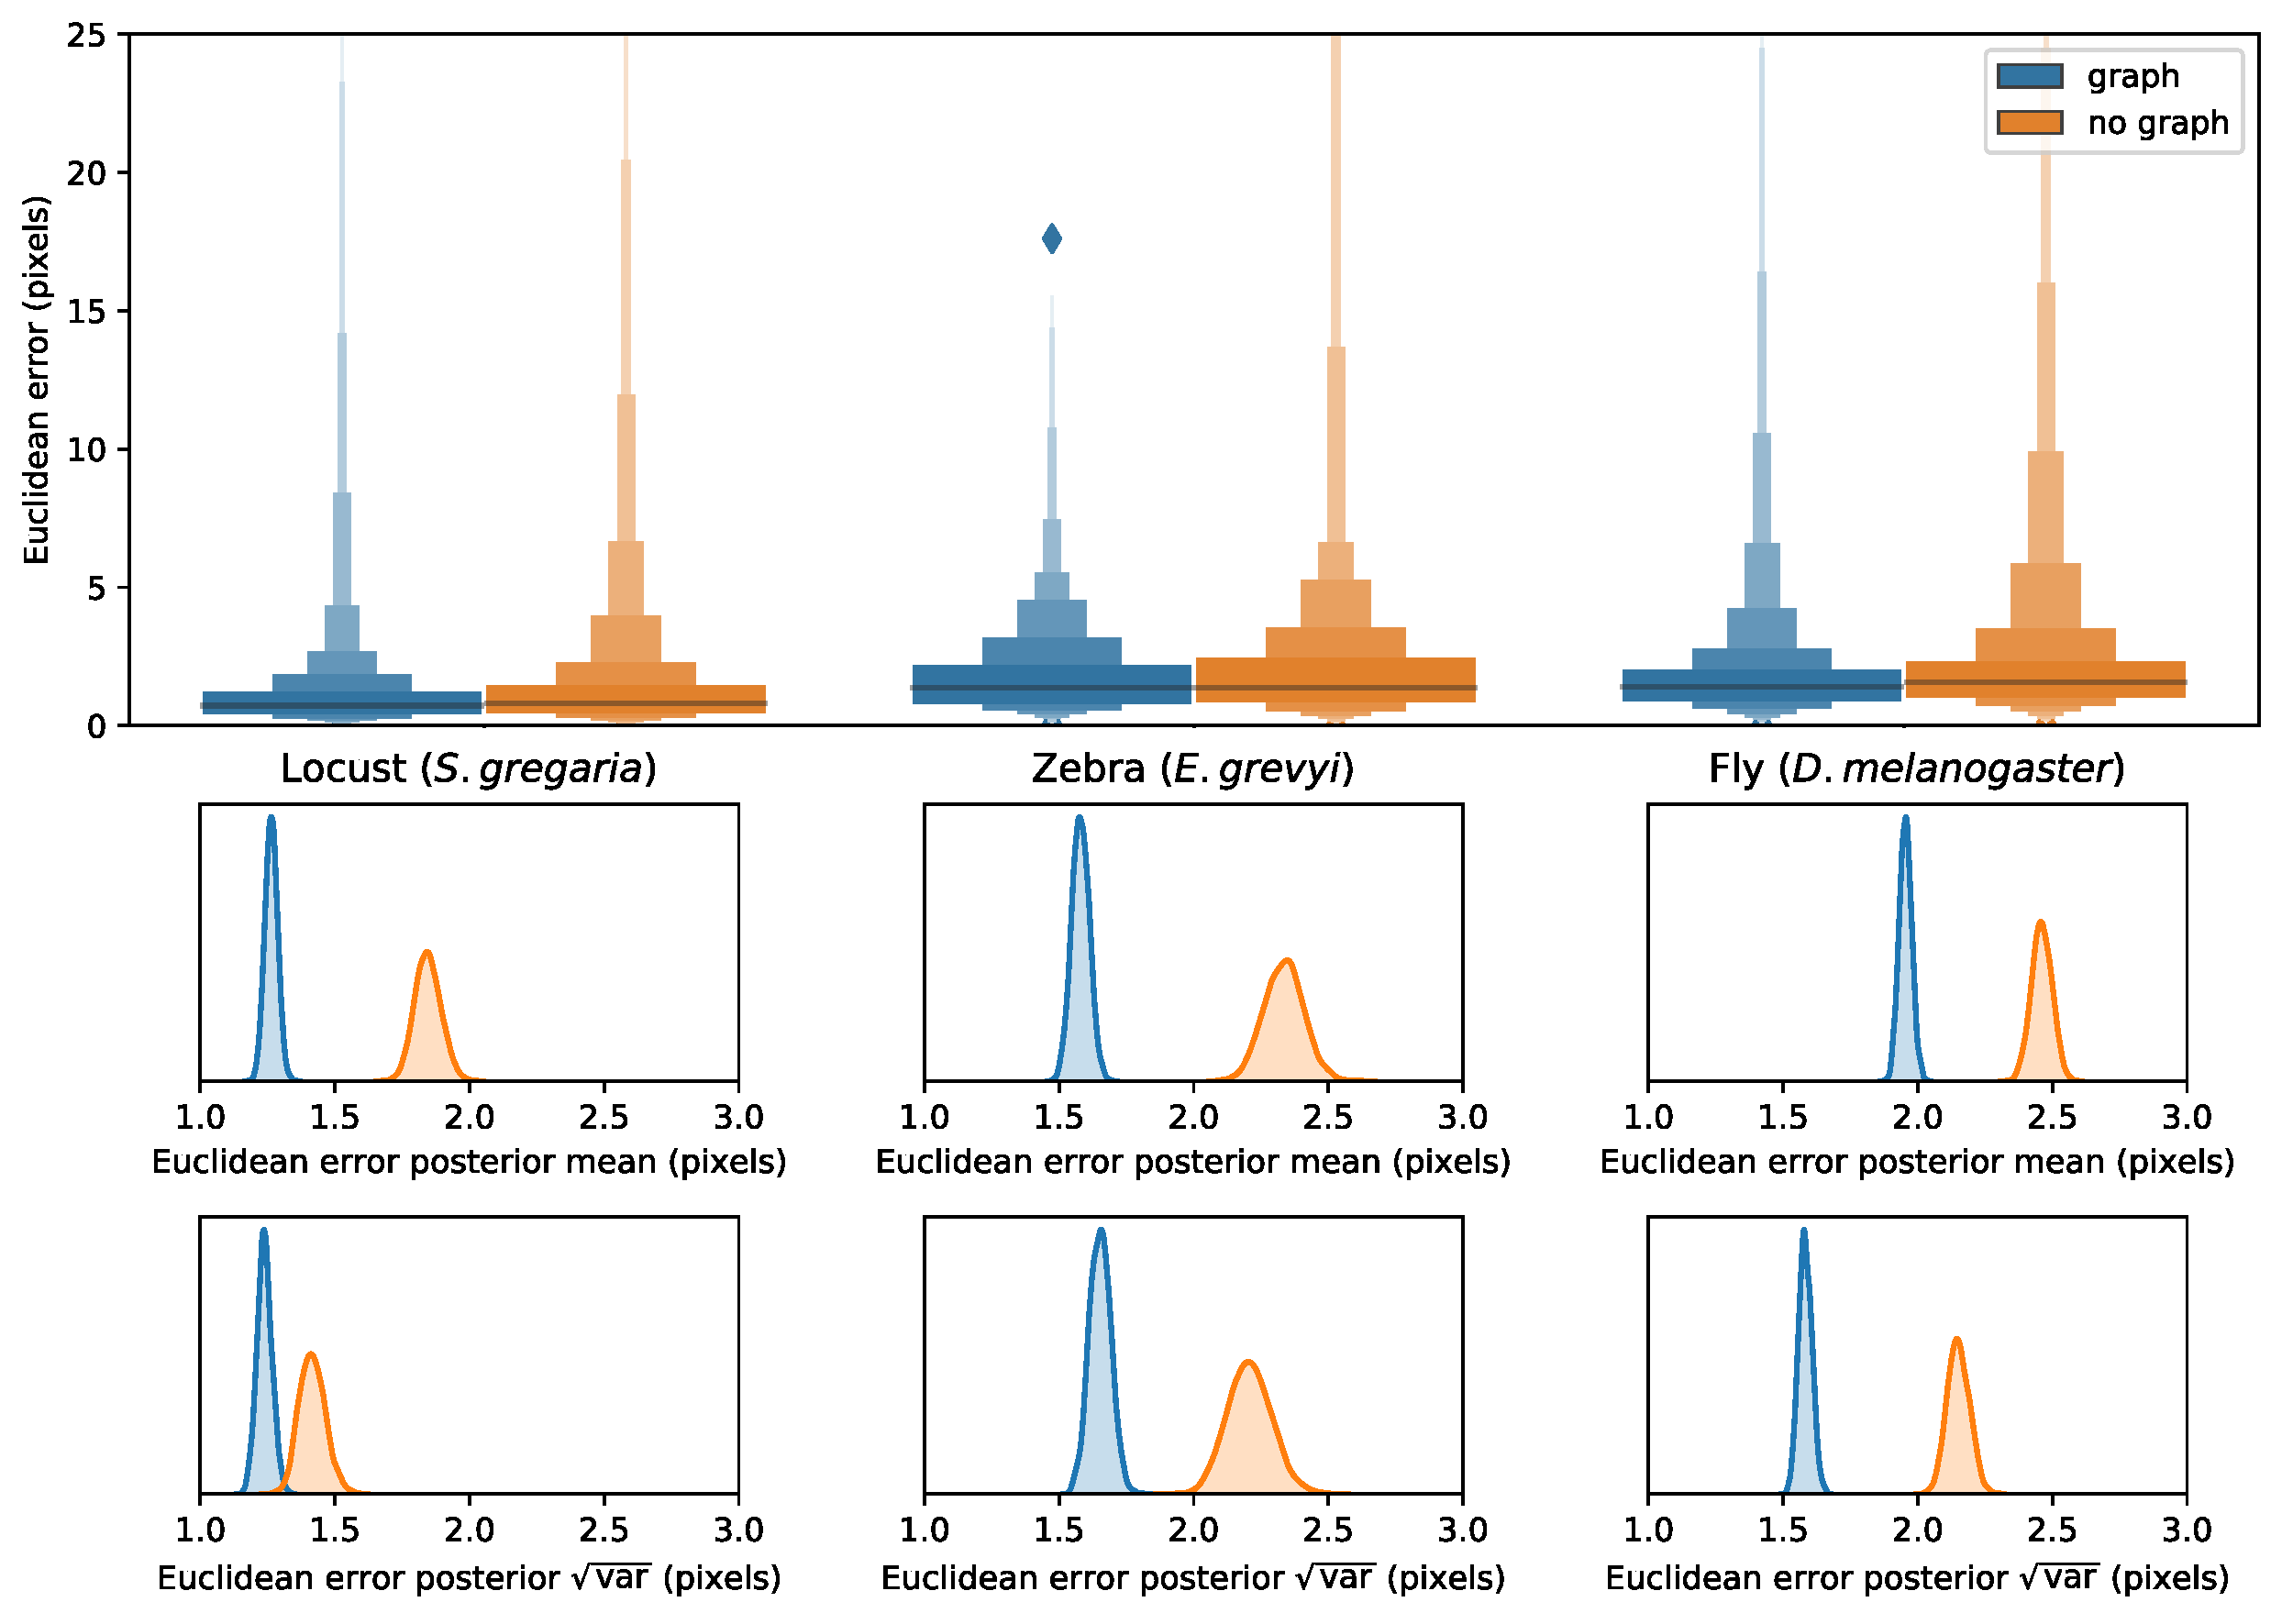
\includegraphics[width=0.76\linewidth]{Graving_IMPRS_Thesis/figures/graph_error_figure.pdf}
    \caption{Predicting the multi-scale geometry of the posture graph reduces error. Letter-value plots (\textbf{top}) show the raw error distributions for each experiment. Visualizations of the posterior distributions for the mean and variance (\textbf{bottom}) show statistical differences between the error distributions. Predicting the posture graph decreases both the mean and variance of the error distribution.}
    \label{fig:graph_error_figure}
    
    
    
    \end{figure}
    
    \begin{figure}[!htb]
    
    \centering
    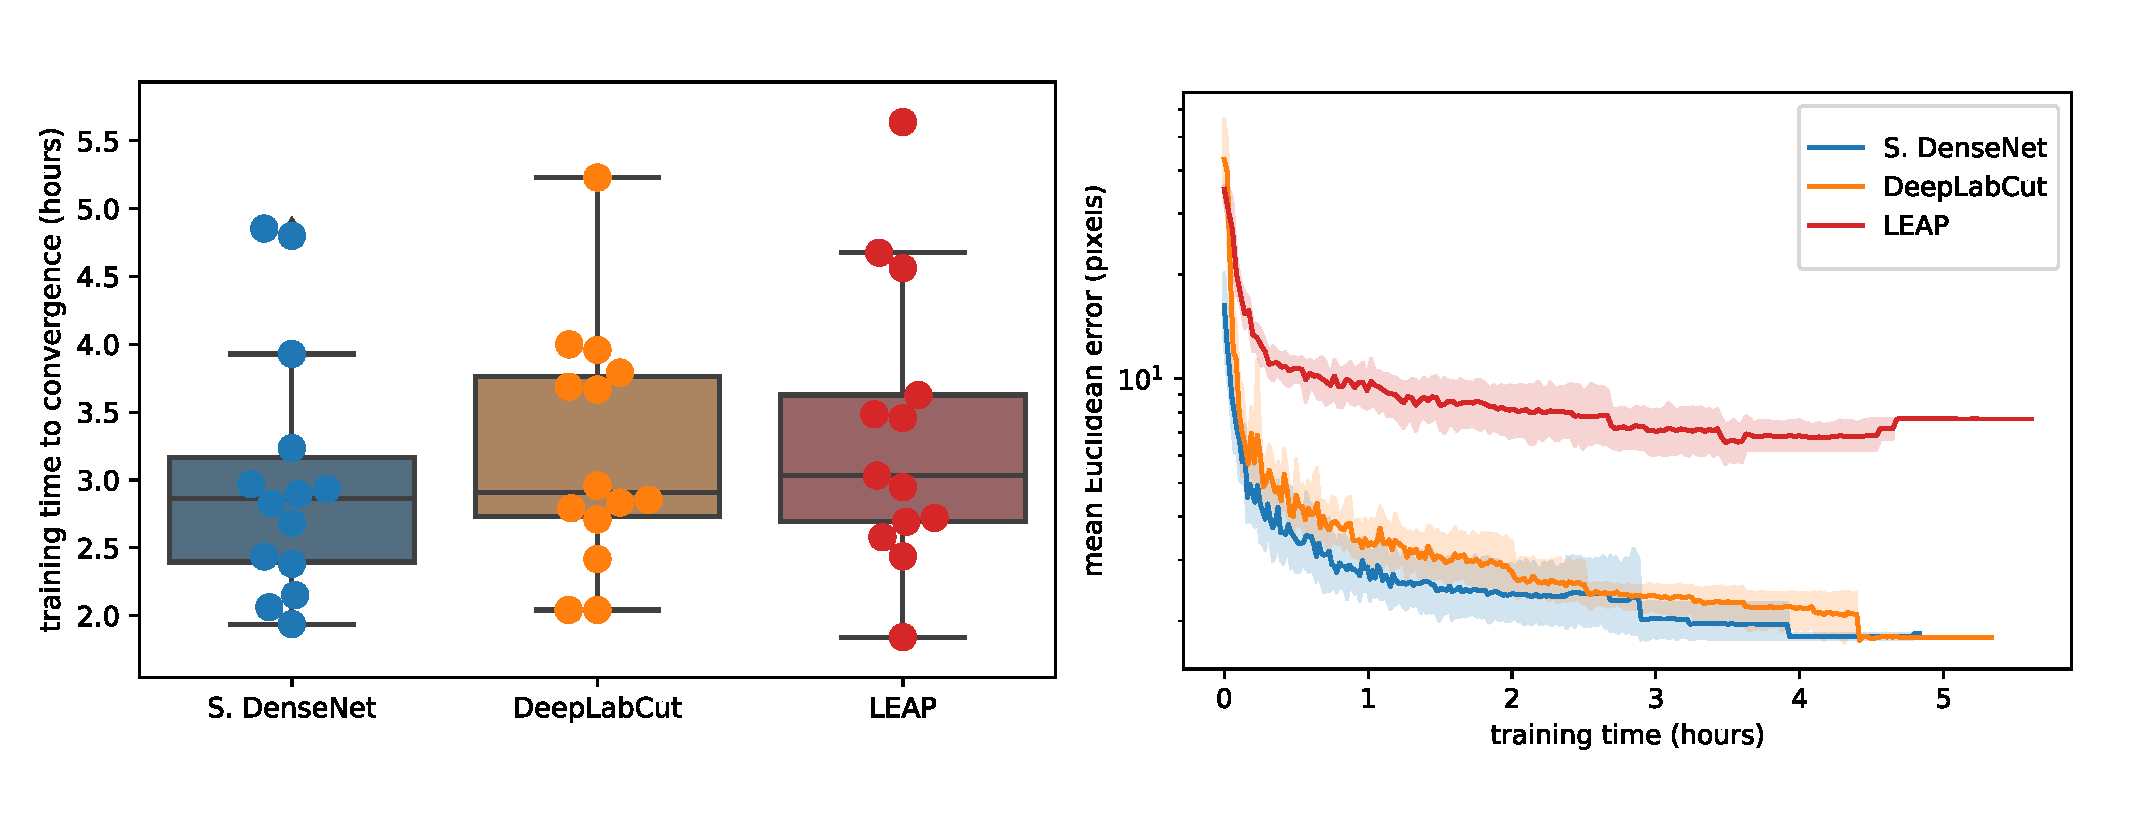
\includegraphics[width=0.8\linewidth]{Graving_IMPRS_Thesis/figures/training_time_figure.pdf}
    \caption{Training time required for our Stacked DenseNet model, the DeepLabCut model \citep{mathis2018deeplabcut}, and the LEAP model \citep{pereira2019fast} (n=15 per model) using our zebra dataset. Boxplots and swarm plots (\textbf{left}) show the total training time to convergence (<0.001 improvement in validation loss for 50 epochs). Line plots (\textbf{right}) illustrate the Euclidean error of the validation set during training, where error bars show bootstrapped (n=1000) 99\% confidence intervals of the mean. Fully training models to convergence requires only a few hours of optimization (\textbf{left}) with reasonable accuracy reached after only 1 hour (\textbf{right}) for our Stacked DenseNet model.}
    \label{fig:training_time}
    
    
    \end{figure}
    
    \begin{figure}[!htb]
    
    \centering
    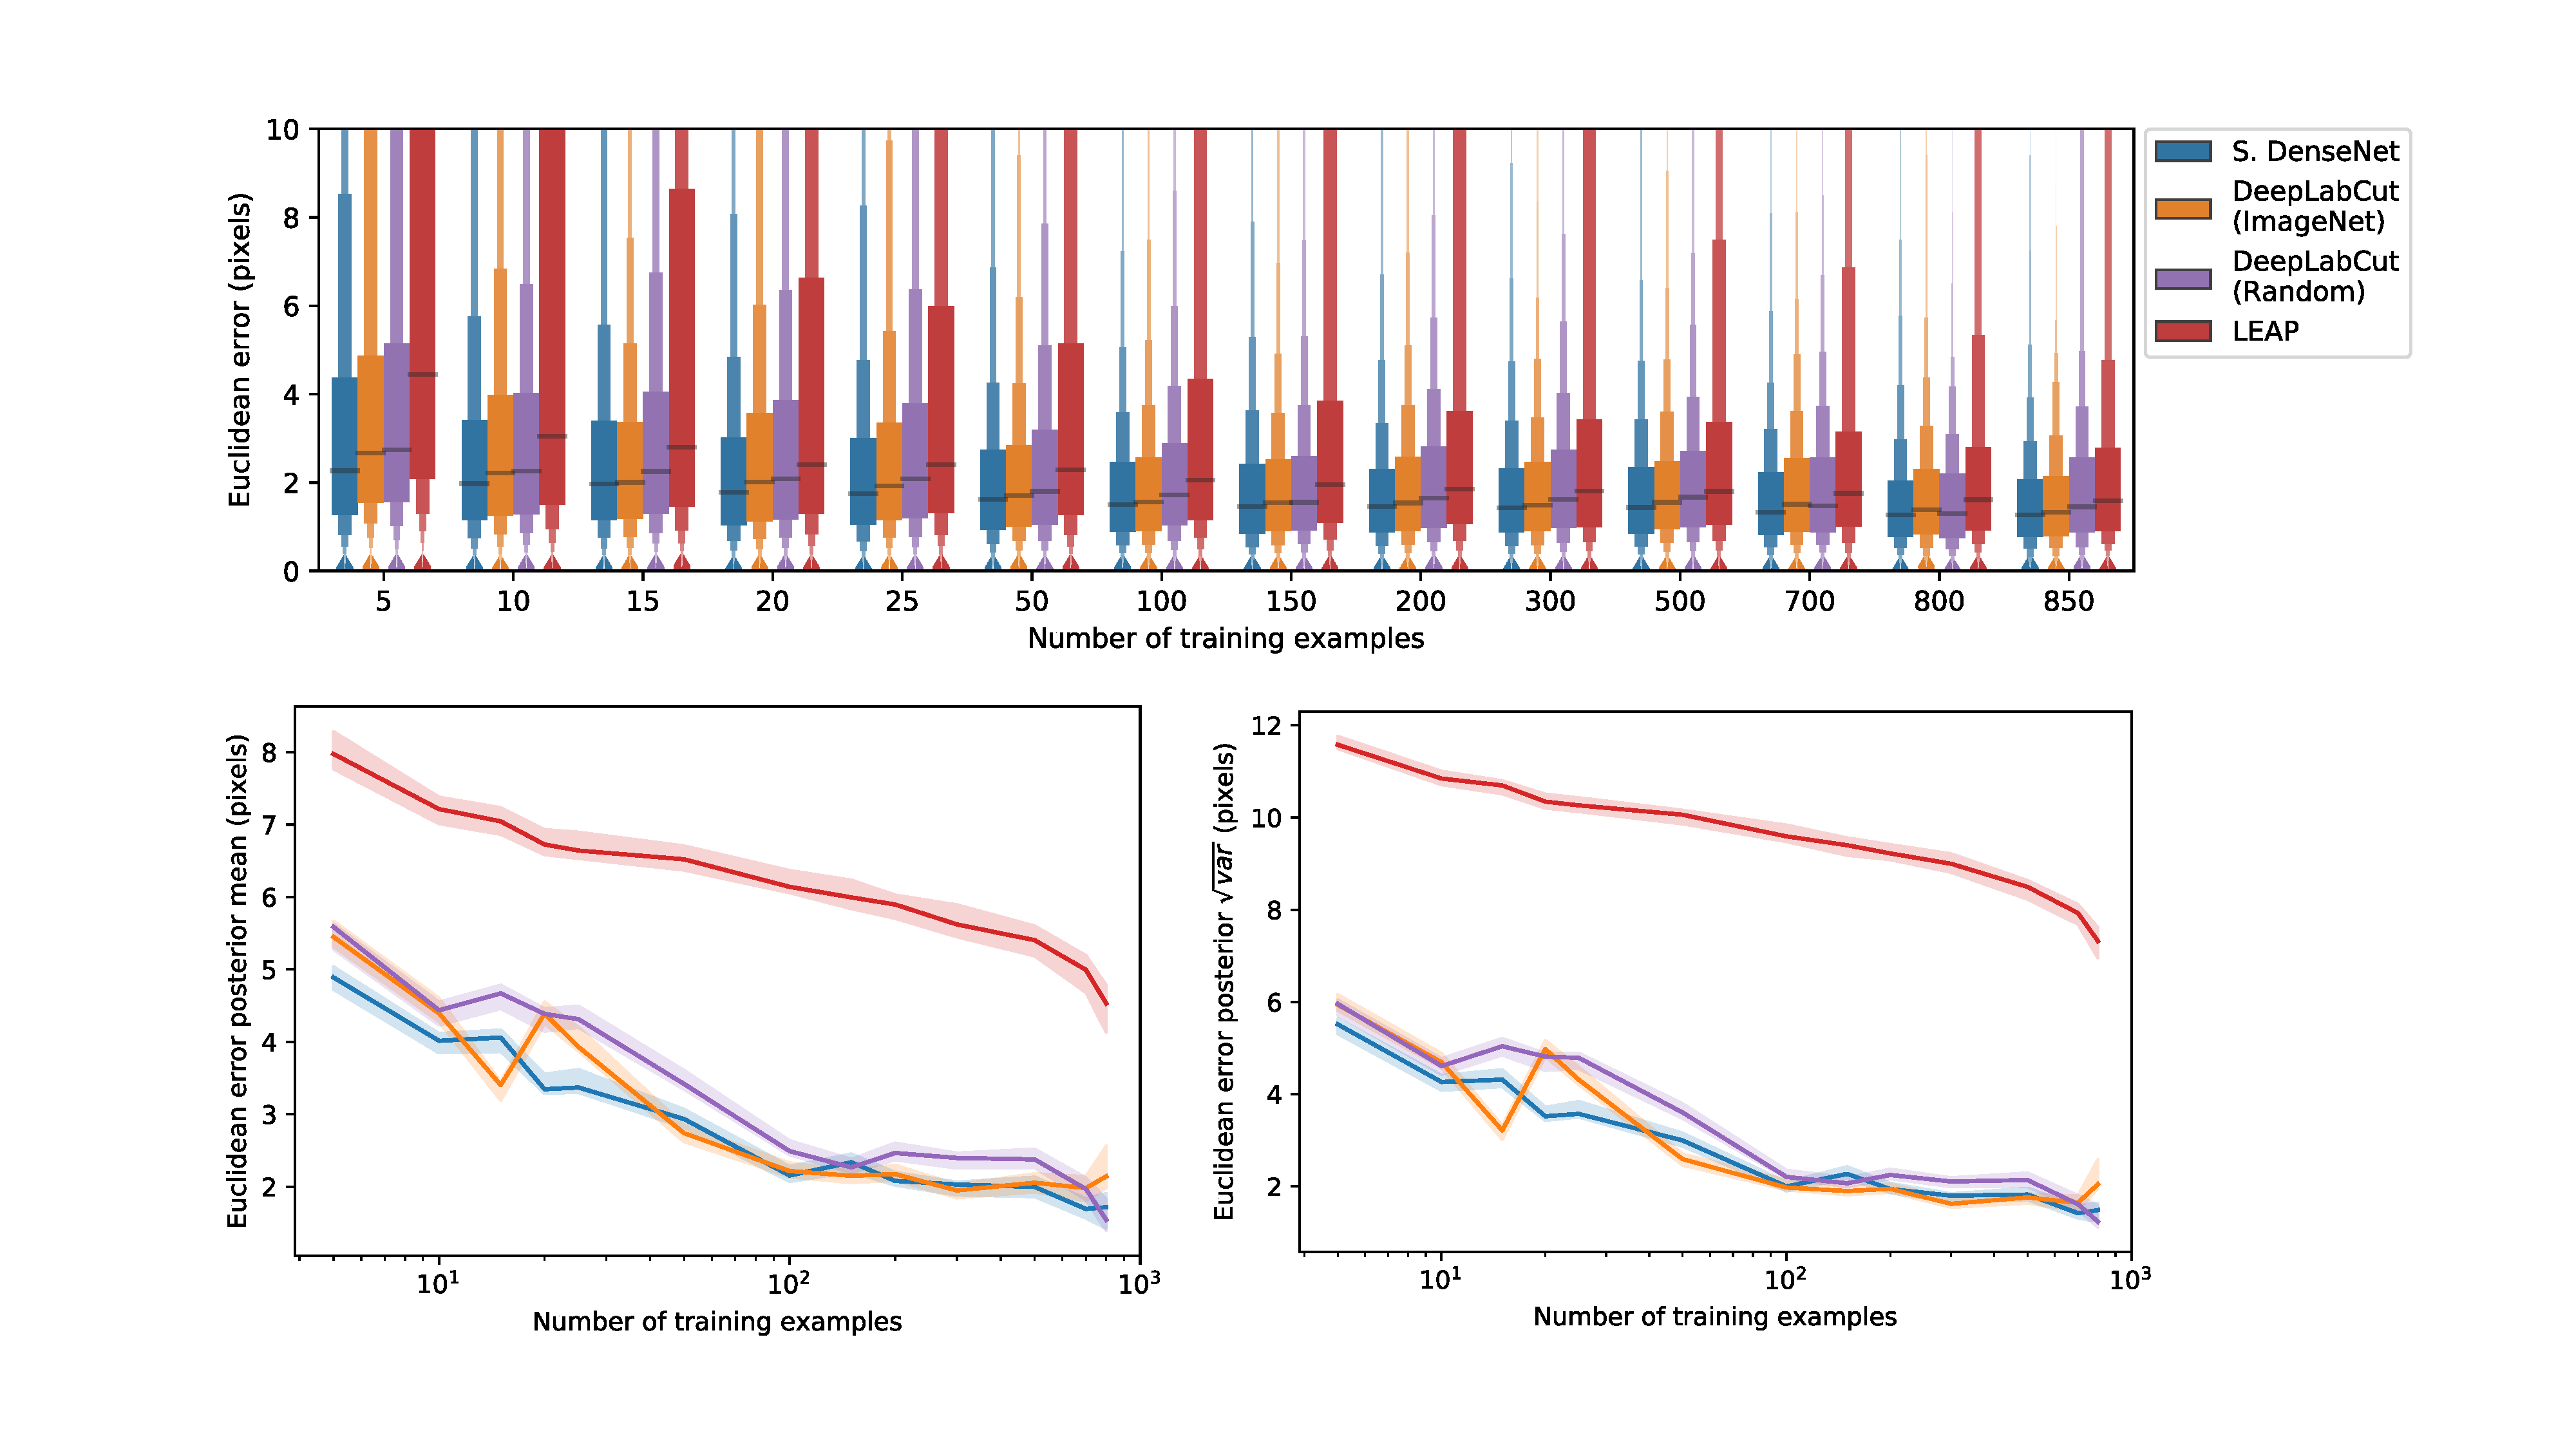
\includegraphics[width=\linewidth]{Graving_IMPRS_Thesis/figures/training_data_proportion_figure.pdf}
    \caption{A comparison of prediction accuracy with different numbers of training examples from our zebra dataset. The error distributions shown as letter-value plots (\textbf{top}) illustrate the Euclidean error for the remainder of the dataset not used for training---with a total of 900 labeled examples in the dataset. Line plots (\textbf{bottom}) show posterior credible intervals (99\% highest-density region) for the mean and variance of the error distributions. We tested our Stacked DenseNet model; the DeepLabCut model \citep{mathis2018deeplabcut} with transfer learning---i.e., with weights pretrained on ImageNet \citep{deng2009imagenet}; the same model without transfer learning---i.e., with randomly-initialized weights; and the LEAP model \citep{pereira2019fast}. Our Stacked DenseNet model achieves high accuracy using few training examples without the use the transfer learning. Using pretrained weights does slightly decrease overall prediction error for the DeepLabCut model \citep{mathis2018deeplabcut}, but the effect size is relatively small.}
    \label{fig:training_prop}
    
    
    \end{figure}
    
    
    
    
    
    %\begin{figure}[!htb]
    %
    %\centering
    %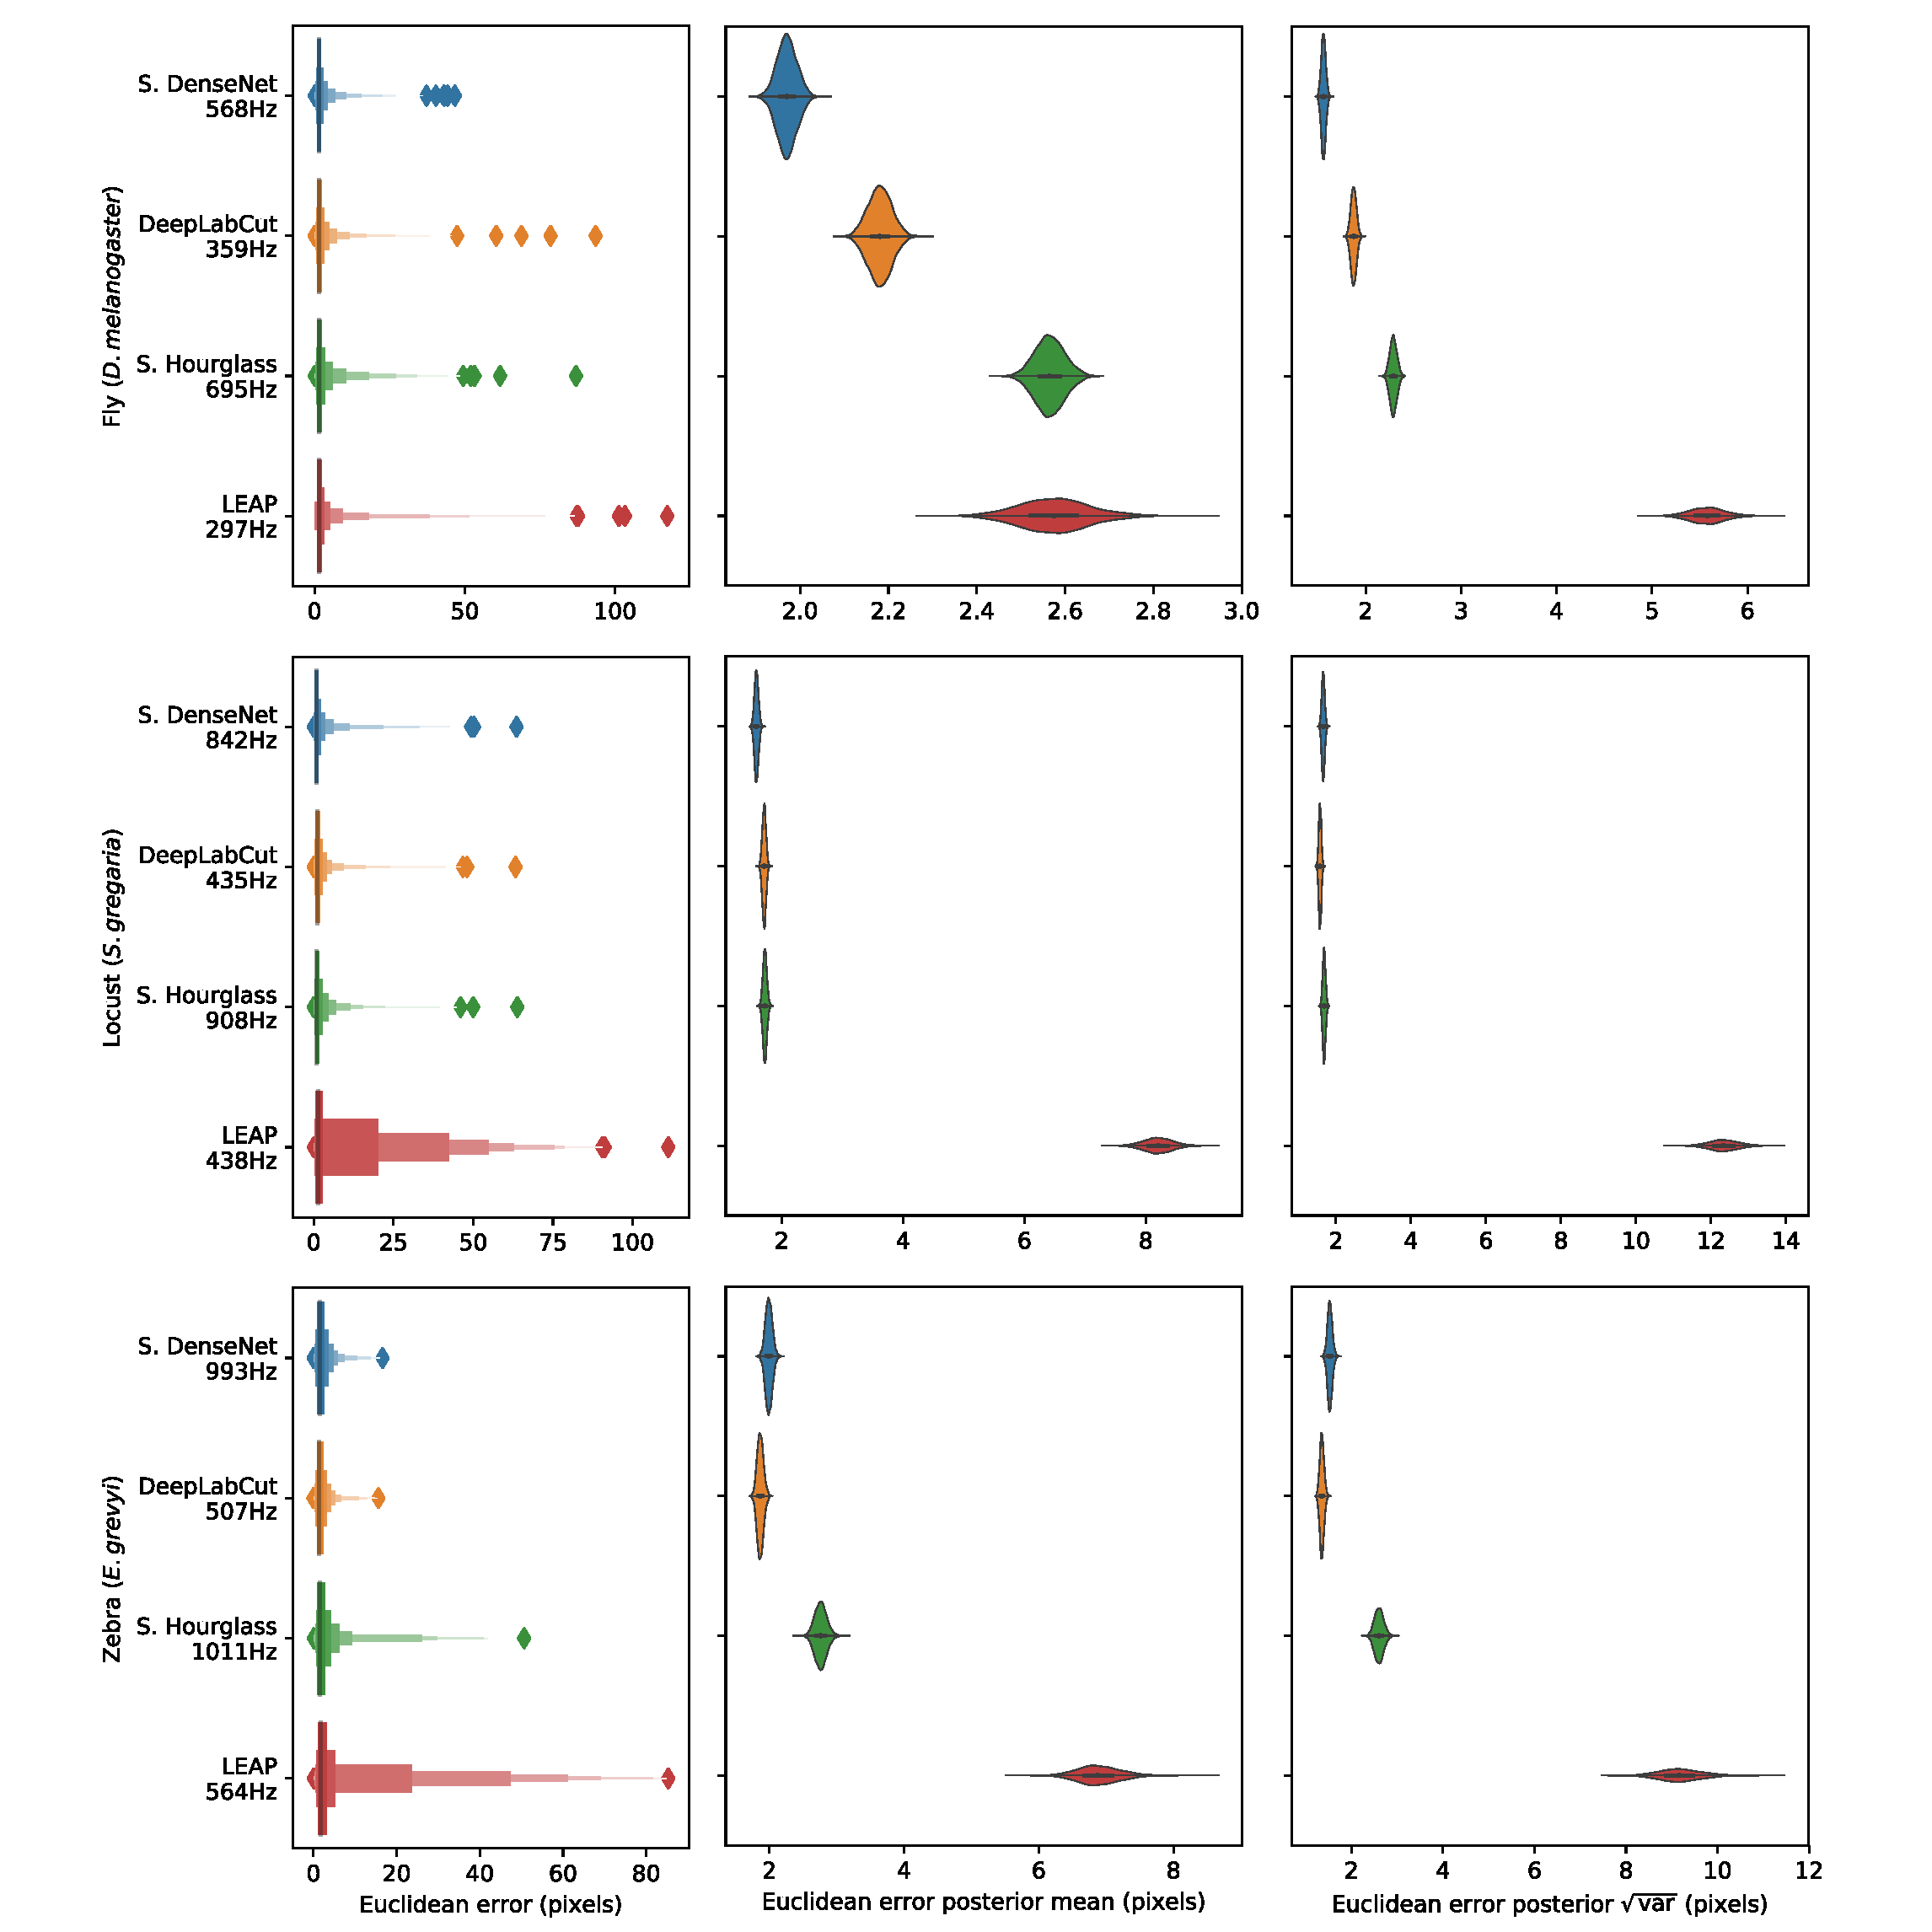
\includegraphics[width=0.75\linewidth]{Graving_IMPRS_Thesis/figures/model_posteriors_figure.pdf}
    %\caption{Euclidean error distributions for each model across our three datasets. Letter-value plots (\textbf{left}) show the raw error distributions for each model. Histograms of the posterior distributions for the mean and variance (\textbf{right}) show statistical differences between the error distributions. Overall the LEAP model \citept{pereira2019fast} was the worst performer on every dataset in terms of both mean and variance. Our implementation of Stacked Densenet was the best performer for the fly dataset, while Stacked DenseNet and DeepLabCut both performed equally well on the locust and zebra datasets. The posteriors for DeepLabCut \citep{mathis2018deeplabcut} and our Stacked DenseNet model are highly overlapping for these datasets, which suggests they are not statistically discernible from one another. The Stacked Hourglass \citep{newell2016} model performed slightly worse than DeepLabCut and our Stacked DenseNet model for all datasets.}
    %\label{fig:model_posteriors_figure}
    %
    %\end{figure}



\section{Convolutional neural networks (CNNs)}
\label{app:cnn}
\textit{Artificial neural networks} like CNNs are complex, non-linear regression models that "learn" a hierarchically–organized set of parameters from real-world data via optimization. These machine learning models are now commonplace in science and industry and have proven to be surprisingly effective for a large number of applications where more conventional statistical models have failed \citep{lecun2015deep}. For computer vision tasks, CNN parameters typically take the form of two-dimensional convolutional filters that are optimized to detect spatial features needed to model relationships between high-dimensional image data and some related variable(s) of interest, such as locations in space—e.g., posture keypoints—or semantic labels \citep{long2015fully,badrinarayanan2017segnet}.

Once a training set is generated (Appendix \ref{app:training_data}), a CNN model must be selected and optimized to perform the prediction task. CNNs are incredibly flexible with regard to how models are specified and trained, which is both an advantage and a disadvantage. This flexibility means models can be adapted to almost any computer vision task, but it also means the number of possible model architectures and optimization schemes is very large. This can make selecting an architecture and specifying hyperparameters a challenging process. However, most research on pose estimation has converged on a set of models that generally work well for this task (Appendix \ref{app:fcnn}).

After selecting an architecture, the parameters of the model are set to an initial value and then iteratively updated to minimize some objective function, or \textit{loss function}, that describes the difference between the model's predictive distribution and the true distribution of the data—in other words, the likelihood of the model's output is maximized. These parameter updates are performed using a modified version of the gradient descent algorithm (\citealt{cauchy1847methode}) known as \textit{mini-batch stochastic gradient descent}—often referred to as simply \textit{stochastic gradient descent} or \textit{SGD} \citep{robbins1951stochastic,kiefer1952stochastic}. SGD iteratively optimizes the model parameters using small randomly-selected subsamples, or \textit{batches}, of training data. Using SGD allows the model to be trained on extremely large datasets in an iterative "online" fashion without the need to load the entire dataset into memory. The model parameters are updated with each batch by adjusting the parameter values in a direction that minimizes the error—where one round of training on the full dataset is commonly referred to as an \textit{epoch}. The original SGD algorithm requires careful selection and tuning of hyperparameters to successfully optimize a model, but modern versions of the algorithm, such as \textit{ADAM} \citep{kingma2014adam}, automatically tune these hyperparameters, which makes optimization more straightforward.

The model parameters are optimized until they reach a convergence criterion, which is some measure of performance that indicates the model has reached a good location in parameter space. The most commonly used convergence criterion is a measure of predictive accuracy—often the loss function used for optimization—on a held-out \textit{validation set}—a subsample of the training data not used for optimization—that evaluates the model's ability to generalize to new "out-of-sample" data. The model is typically evaluated at the end of each training epoch to assess performance on the validation set. Once performance on the validation set stops improving, training is usually stopped to prevent the model from overfitting to the training set—a technique known as \textit{early stopping} \citep{prechelt1998automatic}.



\section{Collecting training data}
\label{app:training_data}

Depending on the variability of the data, CNNs usually require thousands or tens of thousands of manually-annotated examples in order to reach human-level accuracy. However, in laboratory settings, sources of image variation like lighting and spatial scale can be more easily controlled, which minimizes the number of training examples needed to achieve accurate predictions.

This need for a large training set can be further reduced in a number of ways. Two commonly used methods include (1) \textit{transfer learning}—using a model with parameters that are pre-trained on a larger set of images, such as the ImageNet database \citep{deng2009imagenet}, containing diverse features \citep{pratt1993discriminability,insafutdinov2016deepercut, mathis2018deeplabcut}— and (2) \textit{augmentation}— artificially increasing data variance by applying spatial and noise transformations such as flipping (mirroring), rotating, scaling, and adding different forms of noise or artificial occlusions. Both of these methods act as useful forms of \textit{regularization}—incorporating a prior distribution—that allows the model to generalize well to new data even when the training set is small. Transfer learning incorporates prior information that images from the full dataset should contain statistical features similar to other images of the natural world, while augmentation incorporates prior knowledge that animals are bilaterally symmetric, can vary in their body size, position, and orientation, and that noise and occlusions sometimes occur.

\cite{pereira2019fast} introduced two especially clever solutions for collecting an adequate training set. First, they cluster unannotated images based on pixel variance and uniformly sample images from each cluster, which reduces correlation between training examples and ensures the training data are representative of the entire distribution of possible images. Second, they use \textit{active learning} where a CNN is trained on a small number of annotated examples and is then used to initialize keypoint locations for a larger set of unannotated data. These pre-initialized data are then manually corrected by the annotator, the model is retrained, and the unannotated data are re-initialized. The annotator applies this process iteratively as the training set grows larger until they are providing only minor adjustments to the pre-initialized data. This “human-in-the-loop”-style annotation expedites the process of generating an adequately large training set by reducing the cognitive load on the annotator—where the pose estimation model serves as a “cognitive partner”. Such a strategy also allows the annotator to automatically select new training examples based on the performance of the current iteration—where low-confidence predictions indicate examples that should be annotated for maximum improvement (Figure \ref{fig:workflow_figure}).

Of course, annotating image data requires software made for this purpose. \cite{pereira2019fast} provide a custom annotation GUI written in MATLAB specifically designed for annotating posture using an active learning strategy. \cite{mathis2018deeplabcut} recently added a Python-based GUI in an updated version of their software—including active learning and image sampling methods (see \citealt{nath2018}). Our framework also includes a Python-based GUI for annotating data with similar features to \cite{mathis2018deeplabcut} and \cite{pereira2019fast}. 



\section{Fully-convolutional regression}
\label{app:fcnn}

For the task of pose estimation, a CNN is optimized to predict the locations of postural keypoints in an image. One approach is to use a CNN to directly predict the numerical value of each keypoint coordinate as an output. However, making predictions in this way removes real-world constraints on the model's predictive distribution by destroying spatial relationships within images, which negates many of the advantages of using CNNs in the first place.

CNNs are particularly good at transforming one image to produce another related image, or set of images, while preserving spatial relationships and allowing for translation-invariant predictions—a configuration known as a \textit{fully-convolutional neural network} or \textit{F-CNN} \citep{long2015fully}. Therefore, instead of directly regressing images to coordinate values, a popular solution \citep{newell2016, insafutdinov2016deepercut,mathis2018deeplabcut,pereira2019fast} is to optimize a F-CNN that transforms images to predict a stack of output images known as \textit{confidence maps}—one for each keypoint. Each confidence map in the output volume contains a single, two-dimensional, symmetric Gaussian indicating the location of each joint, and the scalar value of the peak indicates the confidence score of the prediction—typically a value between 0 and 1. The confidence maps are then processed to produce the coordinates of each keypoint.

In the case of \textit{multiple pose estimation} where an image contains many individuals, the global geometry of the posture graph is also predicted by training the model to produce \textit{part affinity fields} \citep{cao2017realtime}— directional vector fields drawn between joints in the posture graph—or \textit{pairwise terms} \citep{insafutdinov2016deepercut}—vector fields of the conditional distributions between posture keypoints (e.g., $p(\textrm{foot}|\textrm{head}))$. This allows multiple posture graphs to be disentangled from the image using graph partitioning as the vector fields indicate the probability of the connection between joints (see \citealt{cao2017realtime} for details).


\begin{figure}[!htb]

\begin{center}
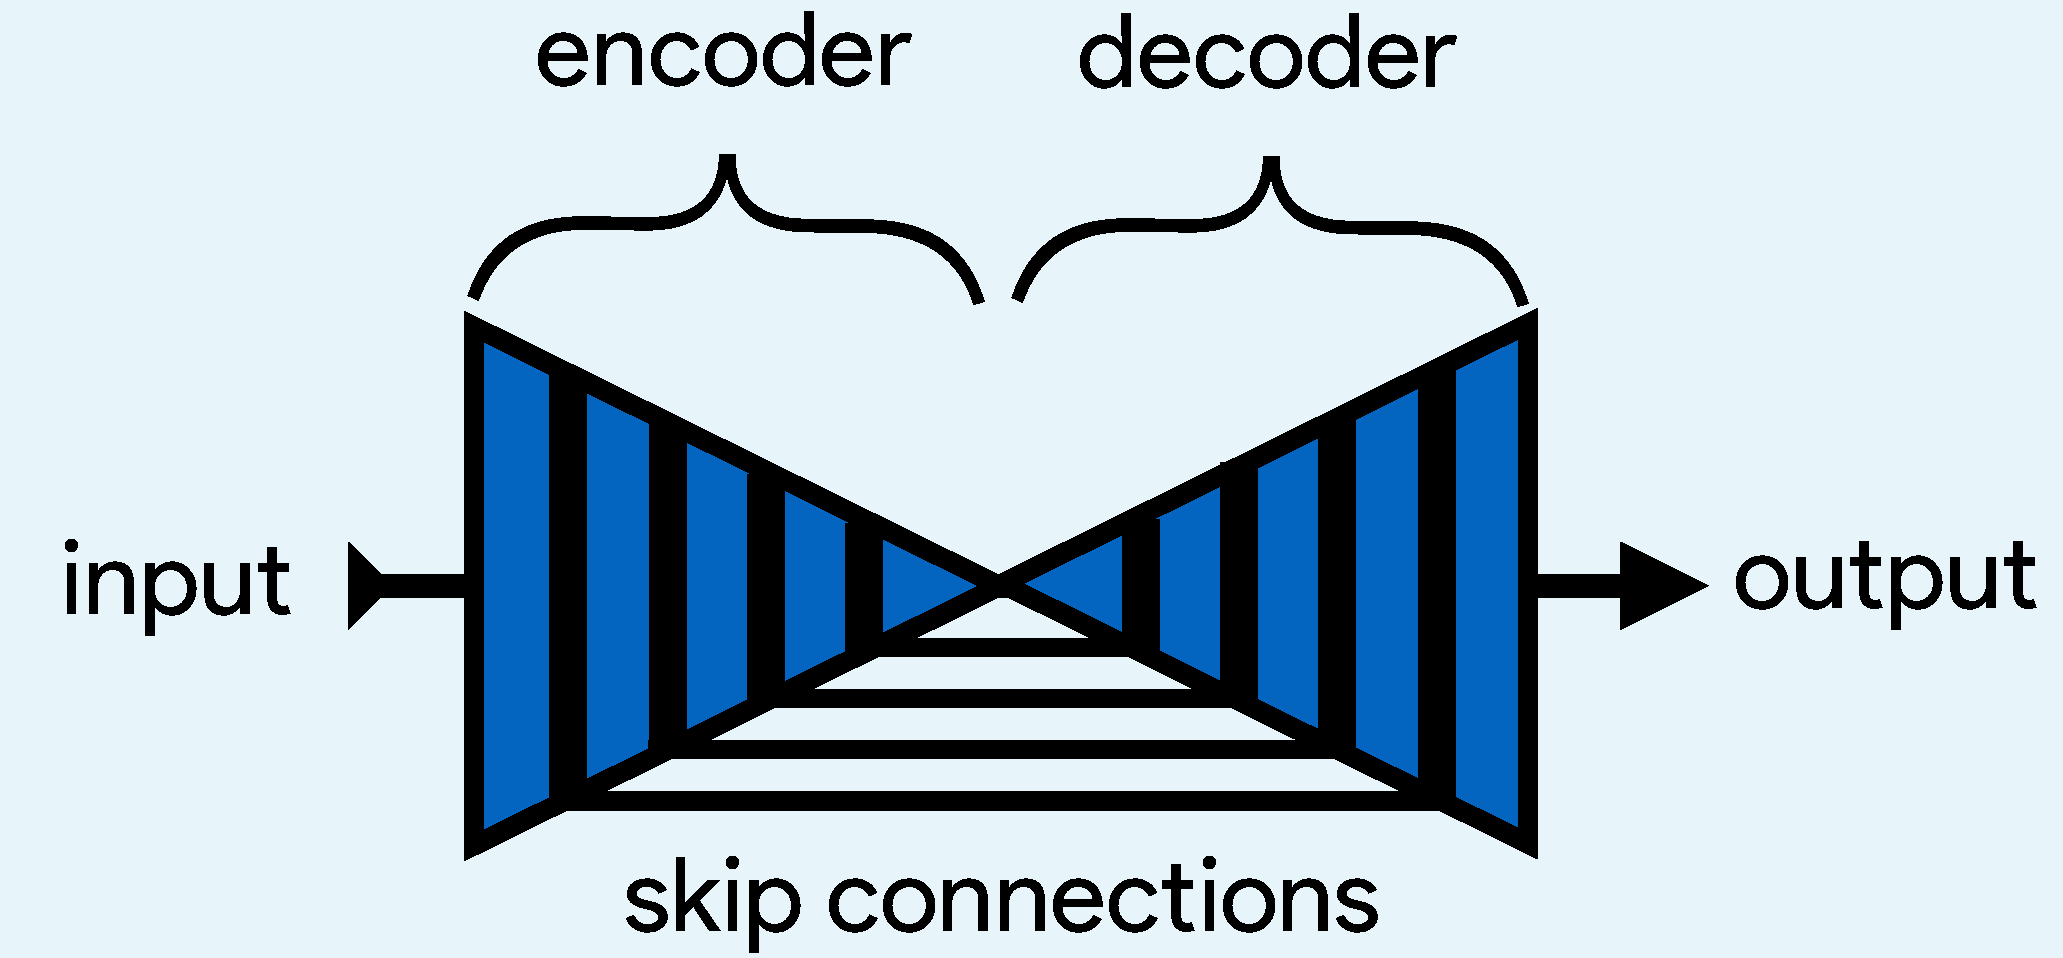
\includegraphics[width=0.5\linewidth]{Graving_IMPRS_Thesis/figures/encoder_decoder_figure.pdf}
\end{center}
\caption{An illustration of the basic encoder-decoder design. The encoder converts the input images into spatial features, and the decoder transforms spatial features to the desired output.}\label{fig:encoder_decoder_figure}
\end{figure}

\section{Encoder-decoder models}
\label{box:encoder_decoder_box}
A popular type of F-CNN (Appendix \ref{app:fcnn}) for solving posture regression problems is known as an \textit{encoder-decoder} model (Figure \ref{fig:encoder_decoder_figure}), which first gained popularity for the task of \textit{semantic segmentation}—a supervised computer vision problem where each pixel in an image is classified into a one of several labeled categories like “dog”, “tree”, or “road” \citep{long2015fully}. This model is designed to repeatedly convolve and downsample input images in the bottom-up \textit{encoder} step and then convolve and upsample the encoder's output in the top-down \textit{decoder} step to produce the final output. Repeatedly applying convolutions and non-linear functions, or \textit{activations}, to the input images transforms pixel values into higher-order spatial features, while downsampling and upsampling respectively increases and decreases the scale and complexity of these features.

\cite{badrinarayanan2017segnet} were the first to popularize a form of this model —known as \textit{SegNet}— for semantic segmentation. However, this basic design is inherently limited because the decoder relies solely on the downsampled output from the encoder, which restricts the features used for predictions to those with the largest spatial scale and highest complexity. For example, a very deep network might learn a complex spatial pattern for predicting “grass” or “trees”, but because it cannot directly access information from the earliest layers of the network, it cannot use the simplest features that plants are green and brown. Subsequent work by \cite{ronneberger2015u} improved on these problems with the addition of \textit{residual} or \textit{skip connections} between the encoder and decoder, where feature maps from encoder layers are concatenated to those decoder layers with the same spatial scale. This set of connections then allows the optimizer, rather than the user, to select the most relevant spatial scale(s) for making predictions.

\cite{Jegou16} are the latest to advance the encoder-decoder paradigm. These researchers introduced a fully-convolutional version of \citeauthor{huang2017densely}’s (\citeyear{huang2017densely}) \textit{DenseNet} architecture known as a \textit{fully-convolutional DenseNet}, or \textit{FC-DenseNet}.  FC-DenseNet’s key improvement is an elaborate set of feed-forward residual connections where the input to each convolutional layer is a concatenated stack of feature maps from all previous layers. This densely-connected design was motivated by the insight that many state-of-the-art models learn a large proportion of redundant features. Most CNNs are not designed so that the final output layers can access all feature maps in the network simultaneously, and this limitation causes these networks to “forget” and “relearn” important features as the input images are transformed to produce the output. In the case of the incredibly popular ResNet-101 \citep{he2016deep} nearly 40\% of the features can be classified as redundant \citep{ayinde2018building}. A densely-connected architecture has the advantages of reduced feature redundancy, increased feature reuse, enhanced feature propagation from early layers to later layers, and subsequently, a substantial reduction in the number of parameters needed to achieve state-of-the-art results \citep{huang2017densely}. Recent work has also shown that DenseNet’s elaborate residual connections have the pleasant side-effect of convexifying the loss landscape during optimization \citep{li2018visualizing}, which allows for faster optimization and increases the likelihood of reaching a good optimum.

\begin{figure}[!htb]

\centering
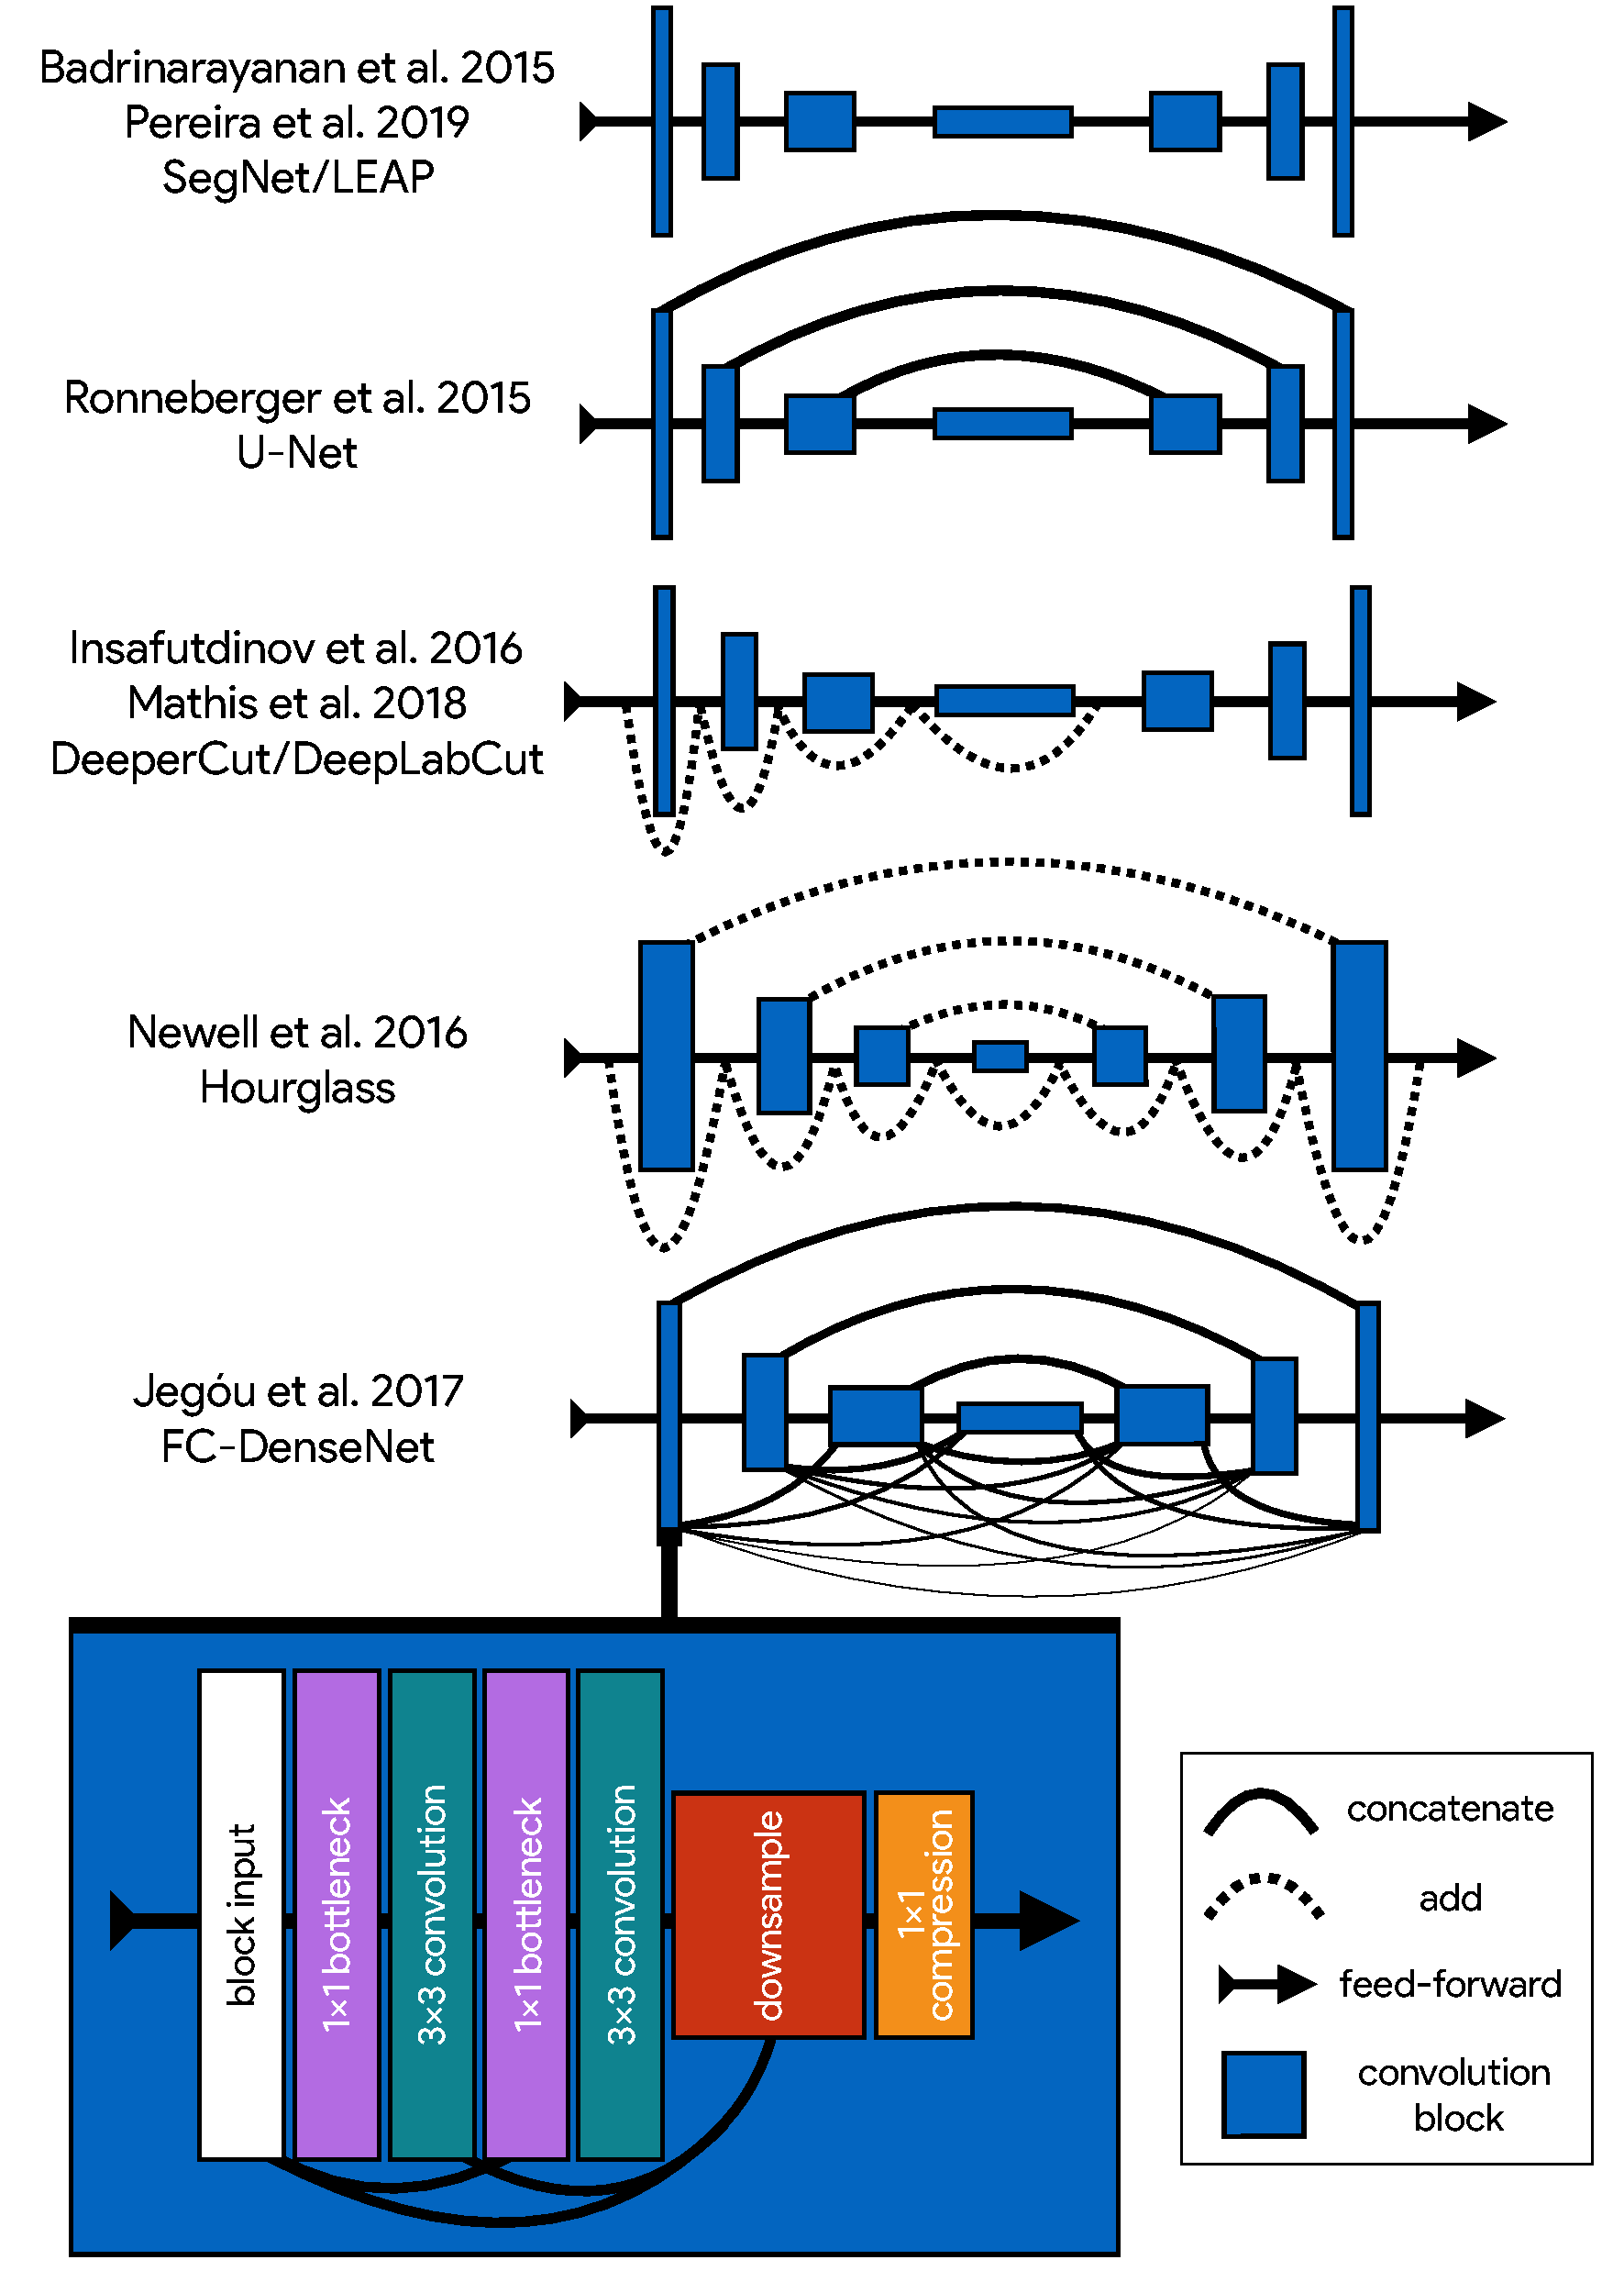
\includegraphics[width=0.75\linewidth]{Graving_IMPRS_Thesis/figures/stacked_densenet_figure.pdf}
\caption{An illustration showing the progression of encoder-decoder architectures from the literature—ordered by performance from top to bottom (see Appendix \ref{app:fcnn} Box \ref{box:encoder_decoder_box} for further details). Most advances in performance have come from adding connections between layers in the network, culminating in FC-DenseNet from \citet{Jegou16}. Lines in each illustration indicate connections between convolutional blocks with the thickness of the line indicating the magnitude of information flow between layers in the network. The size of each convolution block indicates the relative number of feature maps (width) and spatial scale (height). The callout for FC-DenseNet (\citealt{Jegou16}; \textbf{bottom-left}) shows the elaborate set of skip connections within each densely-connected convolutional block as well as our additions of bottleneck and compression layers (described by \citealt{huang2017densely}) to increase efficiency (Appendix \ref{app:implementation})}
\label{fig:stacked_densenet_figure}


\end{figure}

%
%\section{Individual vs. multiple pose estimation}
%\label{app:individual}
%Most recent state-of-the-art methods for posture estimation now focus on simultaneously estimating the pose of multiple individuals in an image (e.g. \citealt{cao2017realtime})—known as \textit{multiple pose estimation}. However, the majority of work on multiple pose estimation has not adequately solved the tracking problem of linking individual data across frames in a video, especially after visual occlusions—although recent work has attempted to address this problem \citep{iqbal2017posetrack, andriluka2018posetrack}. Reliably tracking individuals is important for most behavioral studies, and there are a number of diverse methods already available for solving this problem \citep{perez2014idtracker, crall2015beetag, graving2017pinpoint, romero2018idtracker, wild2018honeybee,boenisch2018tracking}. Additionally, multiple pose estimation requires exhaustively annotating images of multiple individuals—where every individual in the image must be annotated for the model to learn correctly. This type of annotation task is even more laborious and time consuming than annotations for individual pose estimation and increases proportionally with the number of individuals in each frame. Therefore, to avoid solving an already-solved problem of tracking individuals and to circumvent the cognitively complex task of annotating data for multiple pose estimation, the work we describe in this paper is purposefully limited to \textit{individual pose estimation} where each image contains only a single focal individual—which may be localized and cropped from a larger multi-individual image.

%We created a top-down posture estimation framework that can be easily adapted to any data collection workflow, which could include any method for localizing and tracking individuals. This extra step of localizing and tracking individuals, of course, increases the processing time for going from raw images to posture data, which varies depending on the algorithm being used and the number of individuals in each frame. However, increased processing time using automated algorithms is a reasonable trade-off given the alternative of increased manual labor when annotating data—especially considering that the data from most multiple pose estimation algorithms still needs to be linked for each individual across frames to maintain identity. Limiting our methods in this way also simplifies the pose detection problem for designing pose estimation models, which allows for the use of our fast subpixel maxima algorithm on the GPU—as local peak detection is not required. Additionally, because individual pose estimation is such a well-studied problem in computer vision, we can build on the state-of-the-art for this task (see Appendices \ref{app:fcnn} and \ref{app:sota} for details).
%


\label{app:sota}
\section{The state of the art for individual pose estimation}
Many of the current state-of-the-art models for individual posture estimation are based on the design from \cite{newell2016} (e.g., \citealt{Ke_2018_ECCV}, 
\citealt{chen2017adversarial}; also see benchmark results from \citealt{andriluka14cvpr}), but employ various modifications that increase complexity to improve performance. \cite{newell2016} employ what they call a \textit{Stacked Hourglass} network (Appendix \ref{app:fcnn} Figure \ref{fig:stacked_densenet_figure}), which consists of a series of multi-scale encoder-decoder \textit{hourglass} modules connected together in a feed-forward configuration (Figure \ref{fig:model_training_figure}). The main novelties these researchers introduce include (1) stacking multiple hourglass networks together for repeated top-down-bottom-up inference, (2) using convolutional blocks based on the ResNet architecture \citep{he2016deep} with residual connections between the input and output of each block, and (3) using residual connections between the encoder and decoder (similar to \citealt{ronneberger2015u}) with residual blocks in between. \cite{newell2016} also apply a technique known as \textit{intermediate supervision} (Figure \ref{fig:model_training_figure}) where the loss function used for model training is applied to the output of each hourglass as a way of improving optimization across the model's many layers. Recent work by \cite{Jegou16} has further improved on this encoder-decoder design (see Appendix \ref{app:fcnn} Box \ref{box:encoder_decoder_box} and Appendix \ref{app:fcnn} Figure \ref{fig:stacked_densenet_figure}), but to the best of our knowledge, the model introduced by \cite{Jegou16} has not been previously applied to pose estimation.



\label{app:overparam}
\section{Overparameterization and the limitations of LEAP}
Overparameterization is a key limitation for many pose estimation methods, and addressing this problem is critical for high-performance applications. \cite{pereira2019fast} approached this problem by designing their LEAP model after the model from \cite{badrinarayanan2017segnet}, which is a straighforward encoder-decoder design (Appendix \ref{app:fcnn}  Figure \ref{fig:stacked_densenet_figure}; Appendix \ref{app:fcnn} Box \ref{box:encoder_decoder_box}). They benchmarked their model on posture estimation tasks for laboratory animals and compared performance with the more-complex Stacked Hourglass model from \cite{newell2016}. They found their smaller, simplified model achieved equal or better median accuracy with dramatic improvements in inference speed up to 185 Hz. However, \cite{pereira2019fast} first rotationally and translationally aligned each image to improve performance, and their reported inference speeds do not include this computationally expensive preprocessing step. Additionally, rotationally and translationally aligning images is not always possible when the background is complex or highly-variable—such as in field settings—or the study animal has a non-rigid body. This limitation makes the LEAP model \citep{pereira2019fast} unsuitable in many cases. While their approach is simple and effective for a multitude of experimental setups, the LEAP model \citep{pereira2019fast} is also implicitly limited in the same ways as \citeauthor{badrinarayanan2017segnet}’s SegNet model (see Appendix \ref{app:fcnn} Box \ref{box:encoder_decoder_box} for details). The LEAP model cannot make predictions using multiple spatial scales and is not robust to data variance such as rotations \citep{pereira2019fast}.





\label{app:bayesian}
\section{Linear model fitting with Stan}
We estimated the joint posterior $p(\theta_{\mu},\theta_{\phi}|X,y)$ for each model using the No-U-Turn Sampler (NUTS; \citealt{hoffman2014nuts}), a self-tuning variant of the Hamiltonian Monte Carlo (HMC) algorithm \citep{duane1987hybrid}, implemented in Stan \citep{Carpenter_stan:a}. We drew HMC samples using 4 independent Markov chains consisting of 1,000 warm-up iterations and 1,000 sampling iterations for a total of 4,000 sampling iterations. To speed up sampling, we randomly subsampled 20$\%$ of the data from each replicate when fitting each linear model, and we fit each model 5 times to ensure the results were consistent. All models converged without any signs of pathological behavior. We performed a posterior predictive check by visually inspecting predictive samples to assess model fit. For our priors we chose relatively uninformative distributions $\theta_{\mu} \sim \mathit{Cauchy}(0, 5)$ and $\theta_{\phi} \sim \mathit{Cauchy}(0, 10)$, but we found that the choice of prior generally did not have an effect on the final result due to the large amount of data used to fit each model.



\label{app:implementation}

\section{Stacked DenseNet}
Our Stacked DenseNet model consists of an initial 7$\times$7 convolutional layer with stride 2, to efficiently downsample the input resolution—following \cite{newell2016}—followed by a stack of densely-connected hourglass networks with intermediate supervision (Appendix \ref{app:sota}) applied at the output of each network. We also include hyperparameters for the bottleneck and compression layers described by \cite{huang2017densely} to make the model as efficient as possible. These consist of applying a 1$\times$1 convolution to inexpensively compress the number of feature maps before each 3$\times$3 convolution as well as when downsampling and upsampling (see \citealt{huang2017densely} and Appendix \ref{app:fcnn} Figure \ref{fig:stacked_densenet_figure} for details).

\section{Model hyperparameters}
For our Stacked Hourglass model we used a block size of 64 filters (64 filters per 3$\times$3 convolution) with a bottleneck factor of 2 (64/2 = 32 filters per 1$\times$1 bottleneck block). For our Stacked DenseNet model we used a growth rate of 48 (48 filters per 3$\times$3 convolution), a bottleneck factor of 1 (1$\times$growth rate = 48 filters per 1$\times$1 bottleneck block), and a compression factor of 0.5 (feature maps compressed with 1$\times$1 convolution to 0.5$m$ when upsampling and downsampling, where $m$ is the number of feature maps). For our Stacked DenseNet model we also replaced the typical configuration of batch normalization and ReLU activations \citep{goodfellow2016deep} with the more recently-developed self-normalizing SELU activation function \citep{klambauer2017self}, as we found this modification increased inference speed. For the LEAP model \citep{pereira2019fast} we used a 1$\times$ resolution output with integer-based global maxima because we wanted to compare our more complex models with this model in the original configuration described by \citet{pereira2019fast}. The LEAP model could be modified to output smaller confidence maps and increase inference speed, but because there is no obvious "best" way to alter the model to achieve this, we forgo any modification. Additionally, applying our subpixel maxima algorithm at high resolution reduces inference speed compared to integer-based maxima, so this would bias our speed comparisons. 

\section{Our implementation of the DeepLabCut model}
Because the DeepLabCut model from \cite{mathis2018deeplabcut} was not implemented in Keras (a requirement for our pose estimation framework), we re-implemented it. Implementing this model directly in our framework is important to ensure model training and data augmentation are identical when making comparisons between models.  As a consequence, our version of this model does not exactly match the description in the paper but is identical except for the output. Rather than using the location refinement maps described by \cite{insafutdinov2016deepercut} and post-processing confidence maps on the CPU, our version of the DeepLabCut model \citep{mathis2018deeplabcut} has an additional transposed convolutional layer to upsample the output to $\frac{1}{4}\times$ resolution and uses our subpixel maxima algorithm.

To demonstrate that our implementation of the DeepLabCut model matches the performance described by \cite{mathis2018deeplabcut}, we compared prediction accuracy between the two frameworks using the odor-trail mouse dataset provided by \cite{mathis2018deeplabcut} (downloaded from \url{https://github.com/AlexEMG/DeepLabCut/}). This dataset consists of 116 images of a freely-moving individual mouse labeled with four keypoints describing the location of the snout, ears, and the base of the tail. See \cite{mathis2018deeplabcut} for further details on this dataset. We trained both models using 95\% training and 5\% validation data and applied data augmentations for both frameworks using the data augmentation procedure described by \cite{nath2018}. We tried to match these data augmentations as best as possible in DeepPoseKit; however, rather than cropping images as described by \cite{nath2018}, we randomly translated the images independently along the horizontal and vertical axis by drawing from a uniform distribution in the range [-100\%, +100\%]---where percentages are relative to the size of each axis. Translating the images in this way should serve the same purpose as cropping them. 

We trained the original DeepLabCut model \citep{mathis2018deeplabcut} using the default settings and recommendations from \cite{nath2018} for 1 million training iterations. See \cite{mathis2018deeplabcut, nath2018} for further details on the data augmentation and training routine for the original implementation of the DeepLabCut model \citep{mathis2018deeplabcut}. For our re-implementation of the DeepLabCut model \citep{mathis2018deeplabcut} we trained the model with the same batch size and optimization scheme described in the "Model training" section. We then calculated the the prediction accuracy on the full data set. We repeated this procedure five times for each model and fit a Bayesian linear model to a randomly selected subset of the evaluation data to compare the results statistically (see Appendix \ref{app:bayesian}). 

These results demonstrate that our re-implementation of and modification to the DeepLabCut model \citep{mathis2018deeplabcut} have little effect on prediction accuracy (Appendix \ref{app:implementation} Figure \ref{fig:dlc_comparison}). We also provide qualitative comparisons of these results in Appendix \ref{app:implementation} Figure \ref{fig:dlc_comparison}-Figure supplement \ref{figsupp:dlc_tsplot} and Appendix \ref{app:implementation} Figure \ref{fig:dlc_comparison}-video \ref{videosupp:dlcsv1}. For these qualitative comparisons, we also added an additional rotational augmentation (drawing from a uniform distribution in the range [-180$\degree$, +180$\degree$)) when training our implementation of the DeepLabCut model \citep{mathis2018deeplabcut} as we noticed this improved generalization to the video for situations where the mouse rotated its body axis. To the best of our knowledge, rotational augmentations are not currently available when using the software from \cite{mathis2018deeplabcut, nath2018}, which demonstrates the flexibility of the data augmentation pipeline \citep{jung2018imgaug} for DeepPoseKit. The inference speed for the odor-trail mouse dataset using our implementation of the DeepLabCut model \citep{mathis2018deeplabcut} is $\sim$49Hz with a batch size of 64 (offline speeds) and $\sim$35Hz with a batch size of 1 (real-time speeds) at full resolution 640$\times$480, which matches well with results from \cite{mathis2018inference} of $\sim$47Hz and $\sim$32Hz respectively. This suggests our modifications did not affect the speed of the model and that our speed comparisons are also reasonable. Because the training routine could be changed for any underlying model---including the new models we present in this paper---this factor is not relevant when making comparisons as long as training is identical for all models being compared, which we ensure when performing our comparisons.

 
\begin{figure}[!htb]
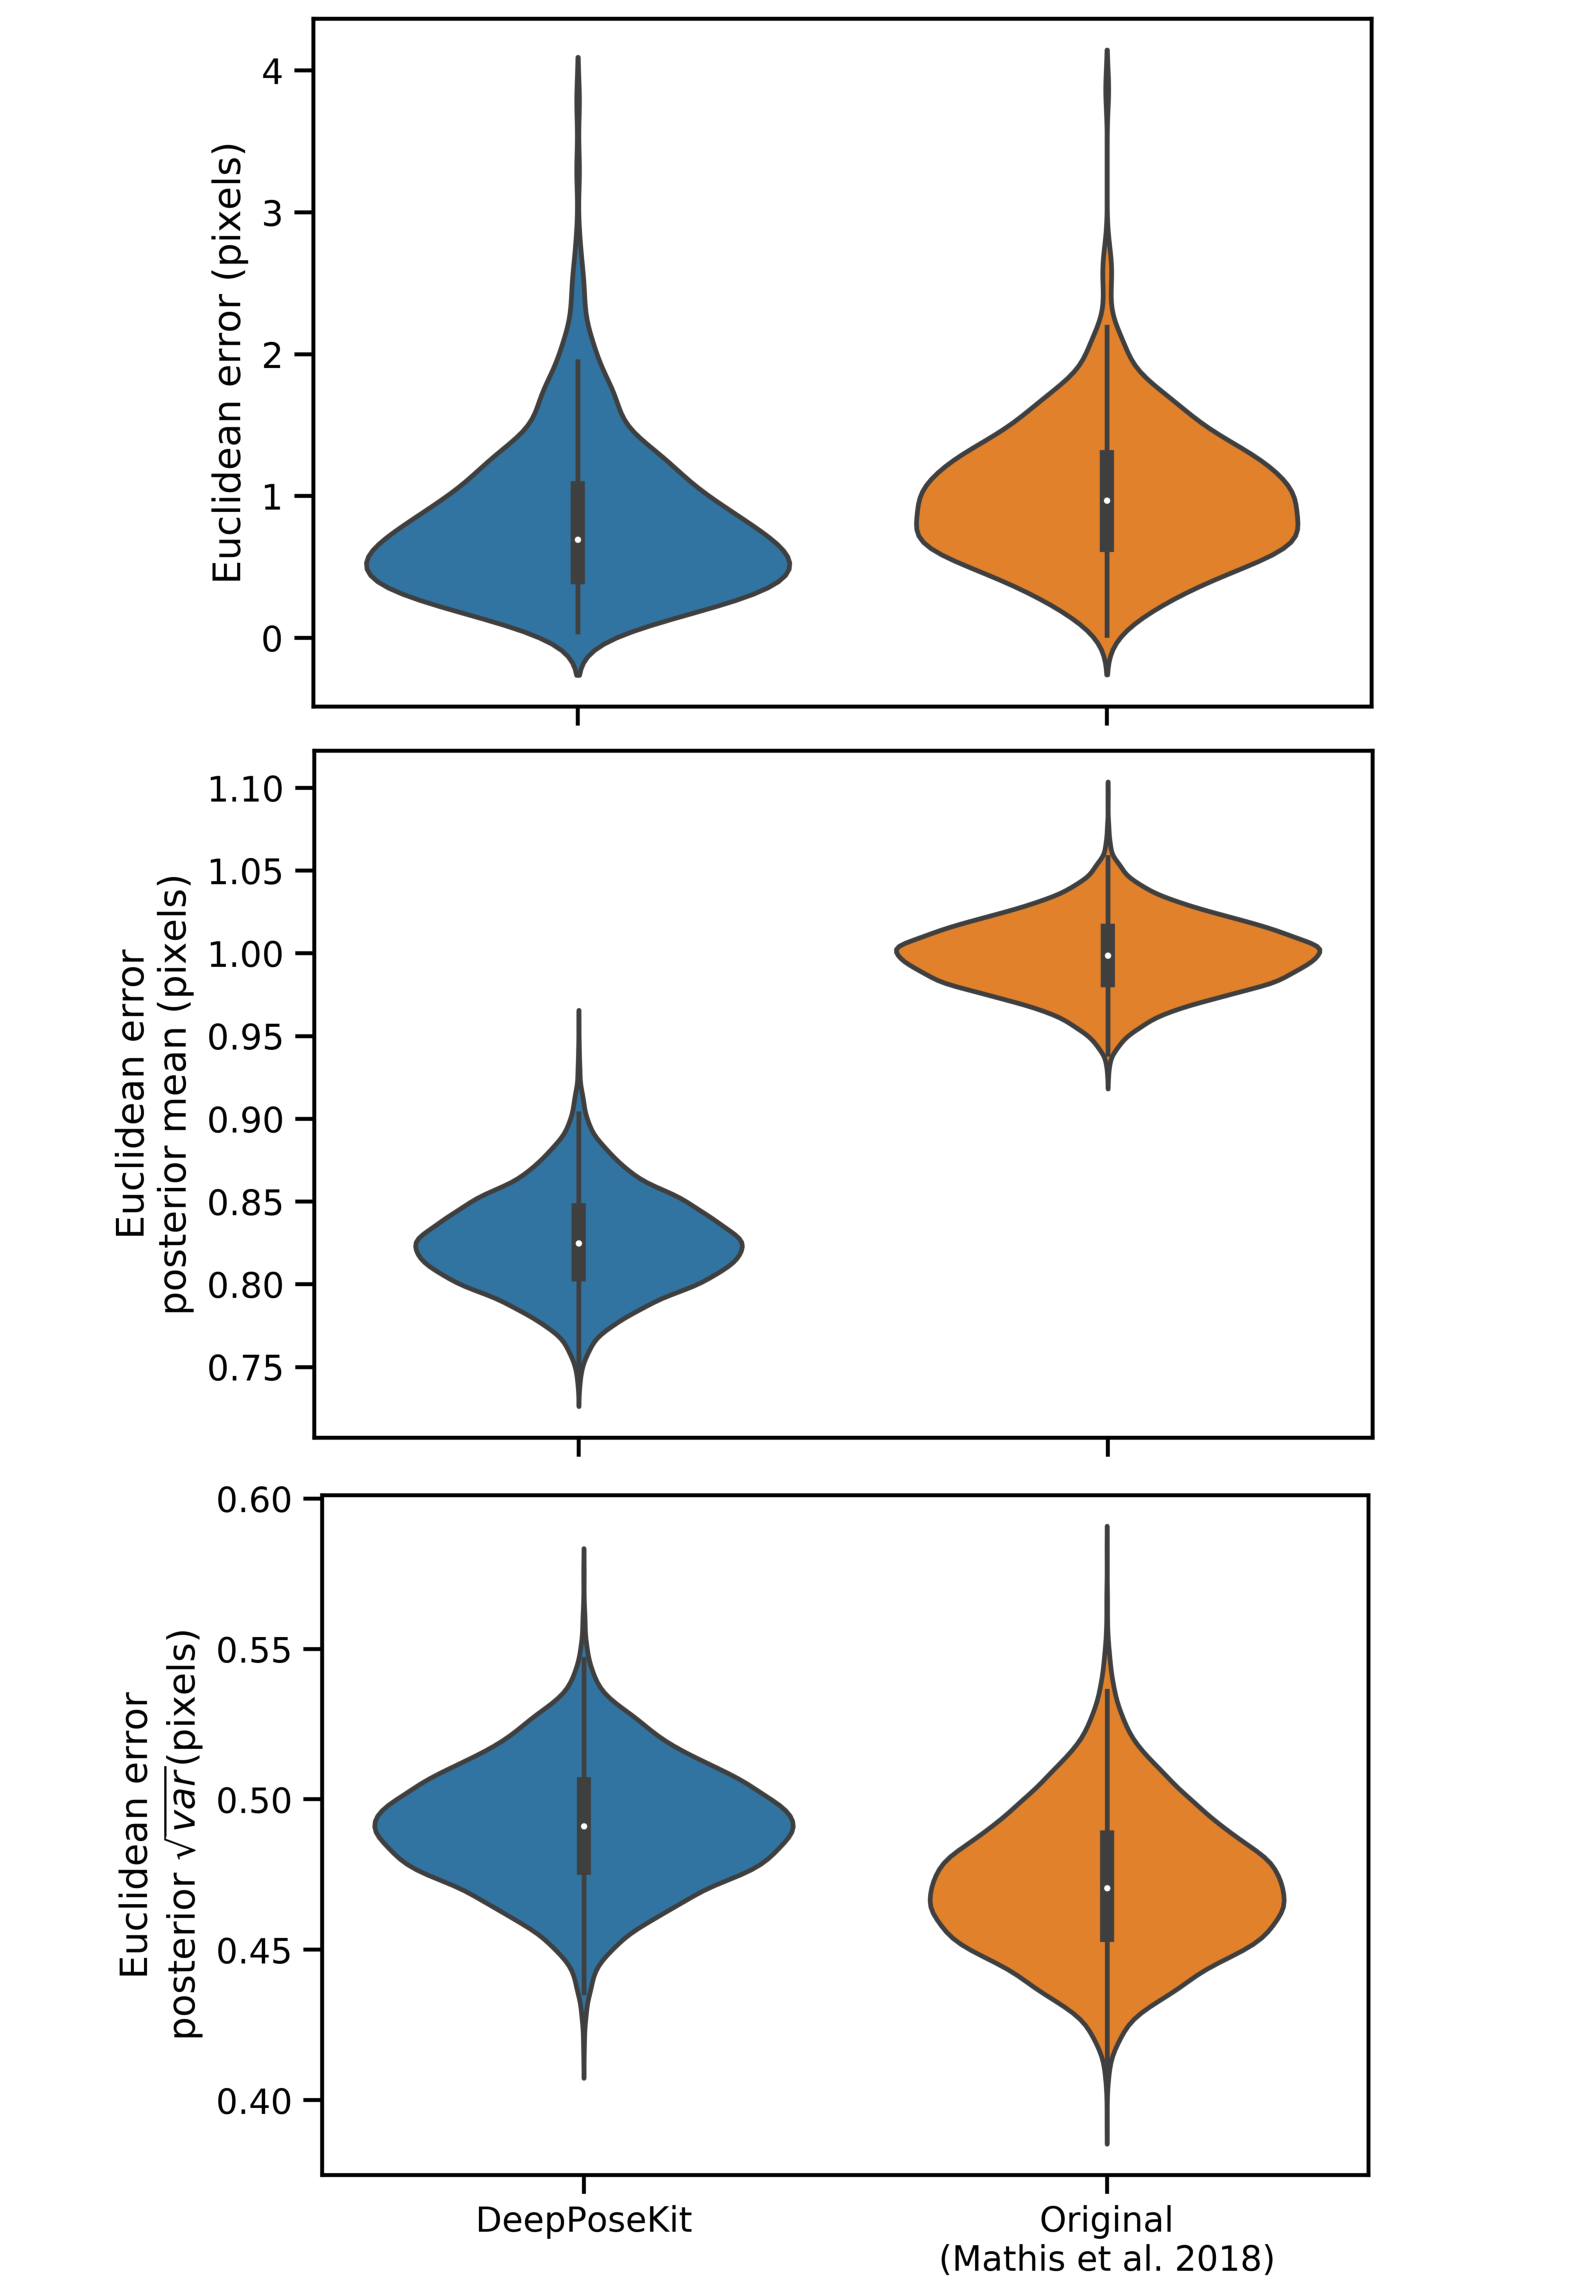
\includegraphics[width=0.8\linewidth]{Graving_IMPRS_Thesis/figures/dlc_comparison_errors.pdf}
\caption{Prediction errors for the odor-trail mouse dataset from \cite{mathis2018deeplabcut} using the original implementation of the DeepLabCut model \citep{mathis2018deeplabcut, nath2018} and our modified version of this model implemented in DeepPoseKit. Mean prediction error is slightly lower for the DeepPoseKit implementation, but there is no discernible difference in variance. These results indicate that the models achieve nearly identical prediction accuracy despite modification. We also provide qualitative comparisons of these results in Appendix \ref{app:implementation} Figure \ref{fig:dlc_comparison}-Figure supplements \ref{figsupp:dlc_tsplot} and \ref{figsupp:dlc_dxtsplot}, and Appendix \ref{app:implementation} Figure \ref{fig:dlc_comparison}-video \ref{videosupp:dlcsv1}.}
\label{fig:dlc_comparison}
\end{figure}

\begin{figure}[!htb]
    \centering
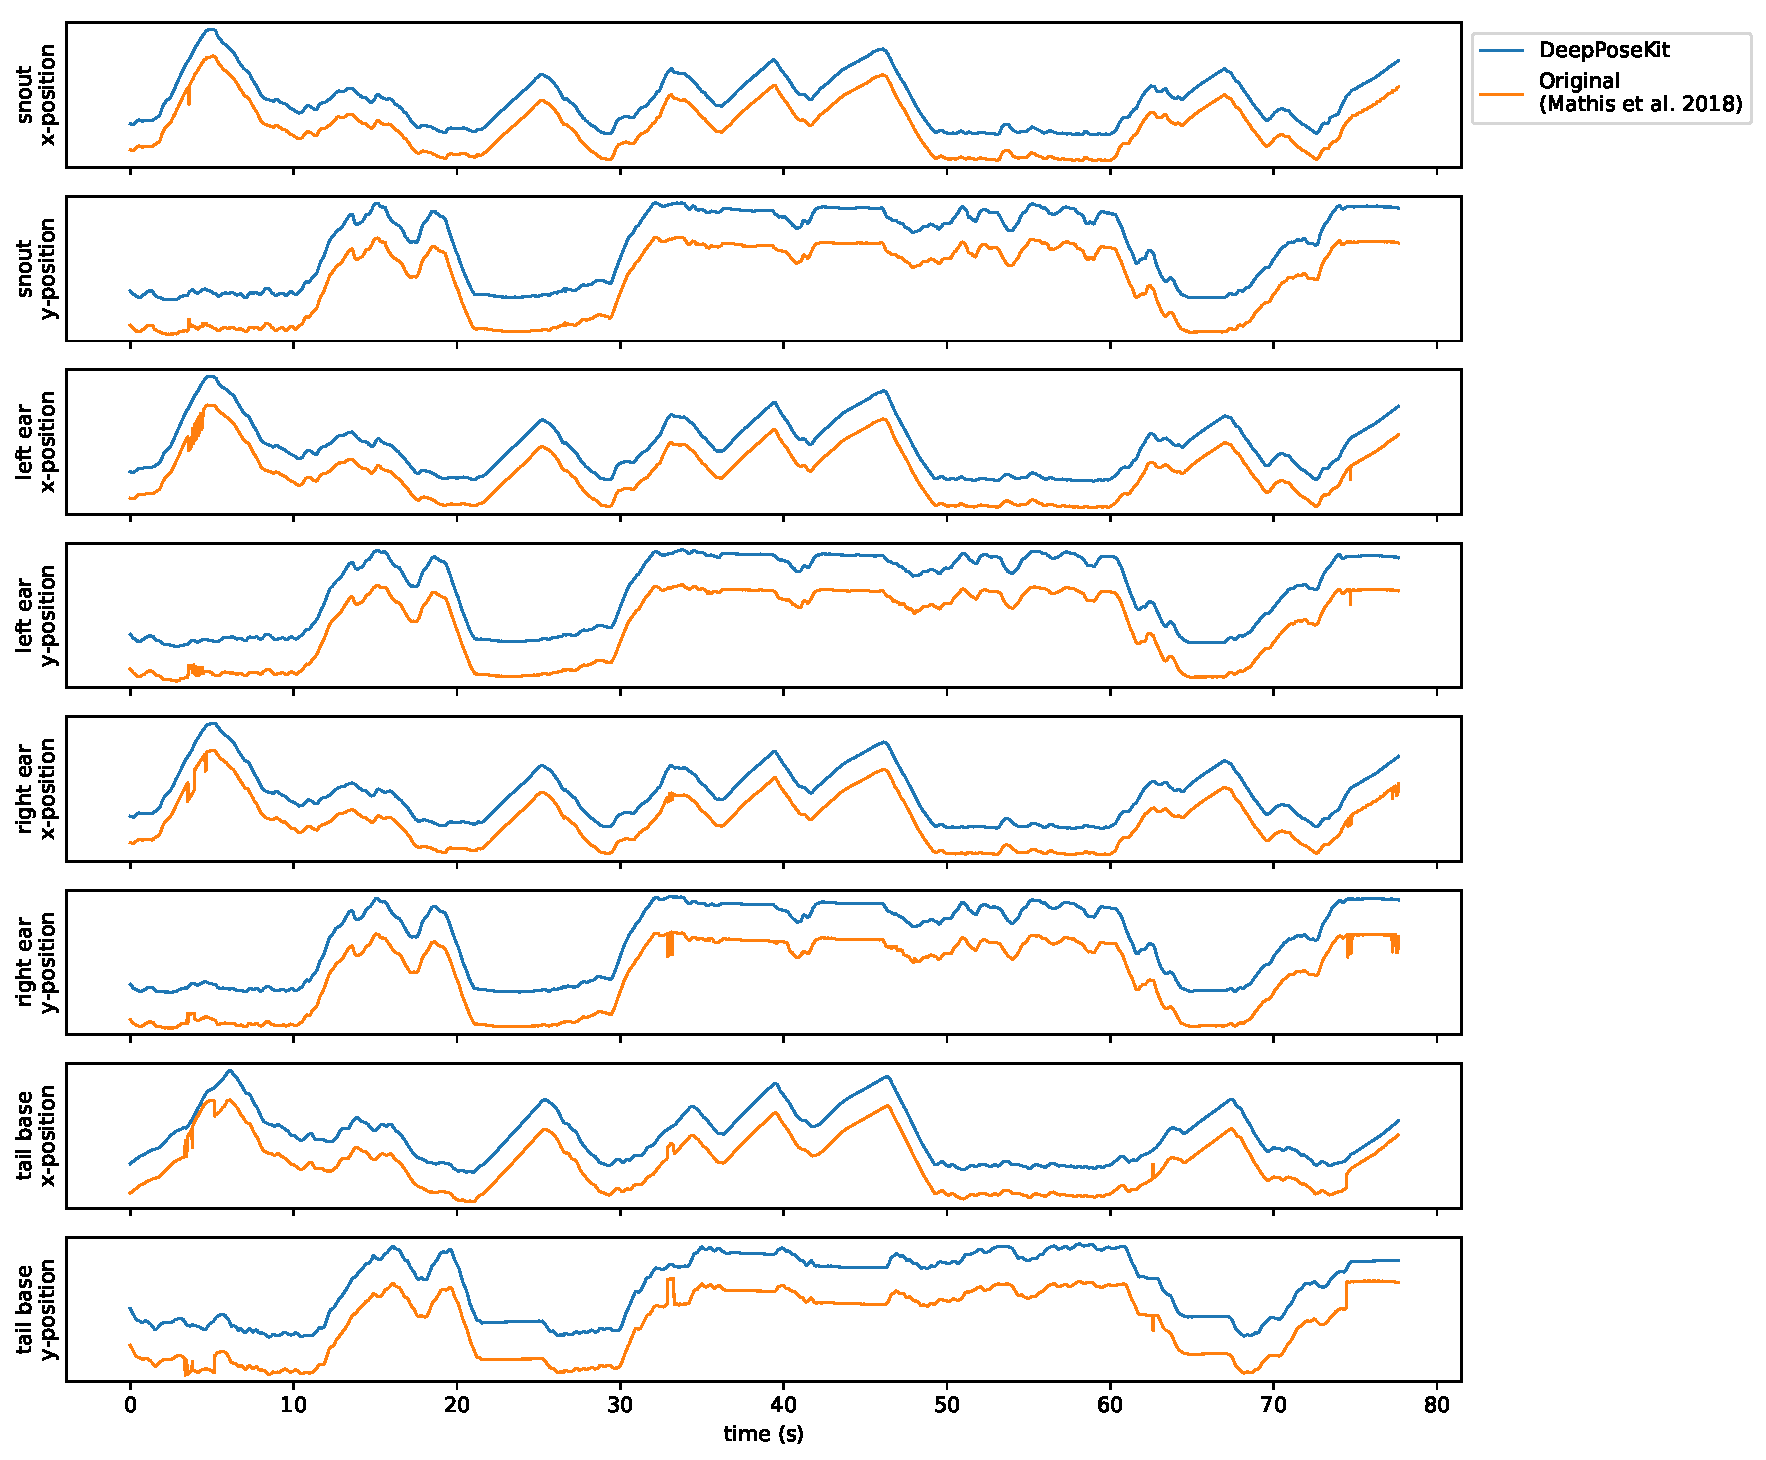
\includegraphics[width=\linewidth]{Graving_IMPRS_Thesis/figures/dlc_tsplot.pdf}    
\caption{Plots of the predicted output for Appendix \ref{app:implementation} Figure \ref{fig:dlc_comparison}-video \ref{videosupp:dlcsv1} comparing our implementation of the DeepLabCut model \citep{mathis2018deeplabcut} in DeepPoseKit vs. the original implementation from \cite{mathis2018deeplabcut, nath2018}. Note the many fast jumps in position for the original verison from \cite{mathis2018deeplabcut}, which indicates prediction errors. }
\label{figsupp:dlc_tsplot}
\end{figure}

\begin{figure}[!htb]
    \centering
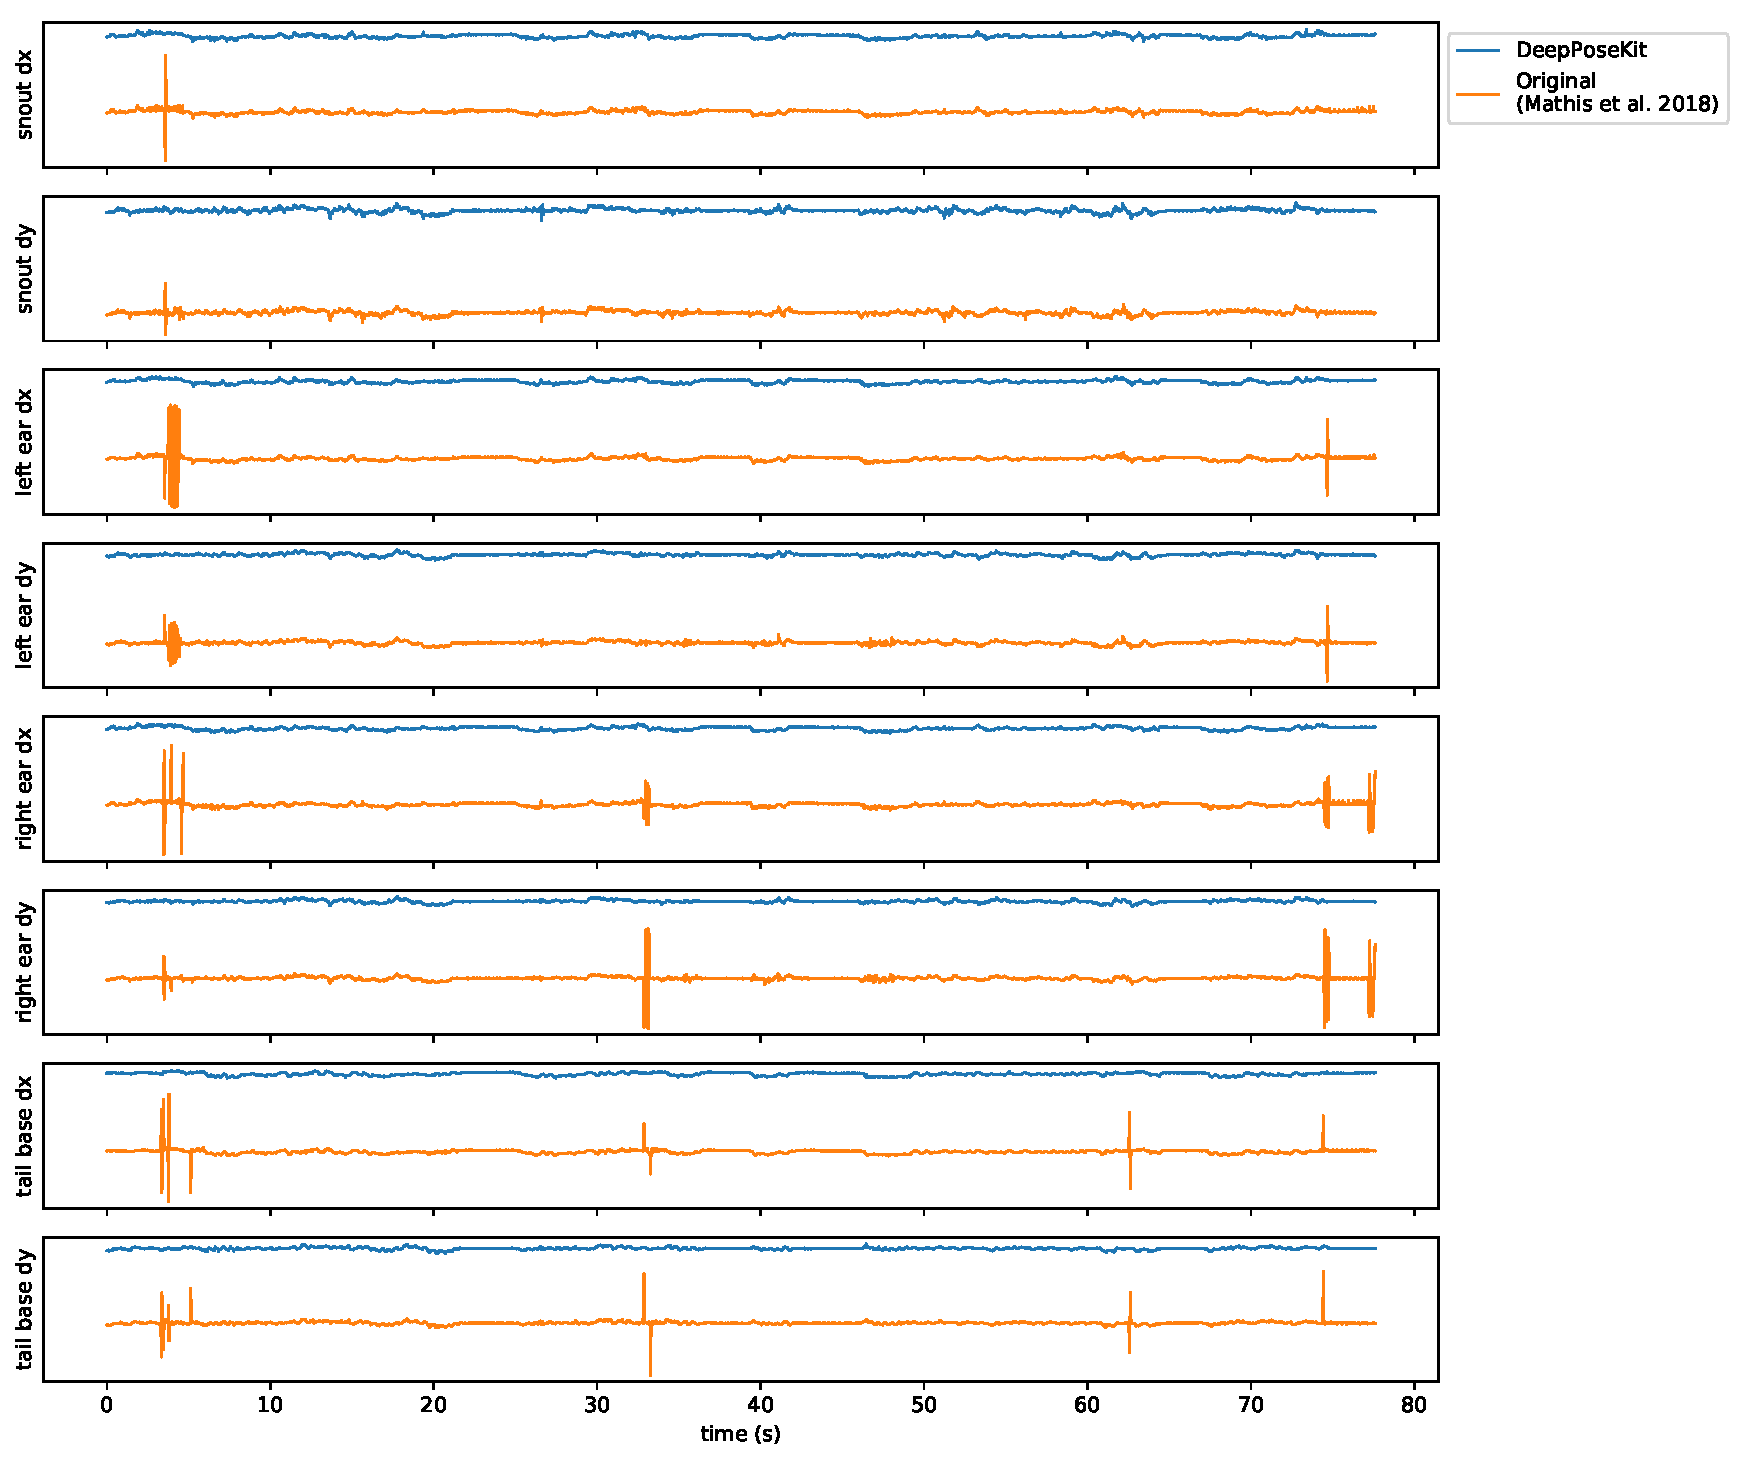
\includegraphics[width=\linewidth]{Graving_IMPRS_Thesis/figures/dlc_dxtsplot.pdf}
\caption{Plots of the temporal derivatives of the predicted output for Appendix \ref{app:implementation} Figure \ref{fig:dlc_comparison}-video \ref{videosupp:dlcsv1} comparing our implementation of the DeepLabCut model \citep{mathis2018deeplabcut} in DeepPoseKit vs. the original implementation from \cite{mathis2018deeplabcut, nath2018}. Note the many fast jumps in position for the original verison from \cite{mathis2018deeplabcut}, which indicates prediction errors}
\label{figsupp:dlc_dxtsplot}
\end{figure}

\begin{figure}[!htb]
    \centering
    \caption{A video comparison of the tracking output of our implementation of the DeepLabCut model \citep{mathis2018deeplabcut} in DeepPoseKit vs. the original implementation from \cite{mathis2018deeplabcut, nath2018}. \url{https://youtu.be/YFmO5C0hUw4}}
\label{videosupp:dlcsv1}
\end{figure}


\label{app:depthwise}
\section[Depthwise-separable convolutions]{Depthwise-separable convolutions for memory-limited applications}
In an effort to maximize model efficiency, we also experimented with replacing 3$\times$3 convolutions in our model implementations with 3$\times$3 depthwise-separable convolutions —first introduced by \cite{chollet2017xception} and now commonly used in fast, efficient “mobile” CNNs (e.g., \citealt{sandler2018mobilenetv2}). In theory this modification should both reduce the memory footprint of the model and increase inference speed. However we found that, while this does drastically decrease the memory footprint of our already memory-efficient models, it slightly decreases accuracy and does not improve inference speed, so we opt for a full 3$\times$3 convolution instead. We suspect that this discrepancy between theory and application is due to inefficient implementations of depthwise-separable convolutions in many popular deep learning frameworks, which will hopefully improve in the near future. At the moment we include this option as a hyperparameter for our Stacked DenseNet model, but we recommend using depthwise-separable convolutions only for applications that require a small memory footprint such as training on a lower-end GPU with limited memory or running inference on a mobile device.
